% $Id: spp-svrp.tex,v 1.40 2006-07-27 18:49:52 jeff Exp $

\documentclass[11pt]{article}
%\documentclass[trsc]{informs1}
%\documentclass[trsc,nonblindrev]{informs1} % for review, not blinded
%\documentclass[trsc,blindrev]{informs1}    % for review, blinded
%\documentclass[opre,copyedit]{informs1}    % spaced for copyediting
%\documentclass[preprint]{elsarticle}    % spaced for copyediting

\usepackage{ifthen}
\def\coralreport{1}

\ifthenelse{\coralreport = 1}{
\usepackage{isetechreport}
\def\reportyear{08T}
\def\reportno{009}
\def\revisionno{1}
\def\originaldate{October 13, 2008}
\def\revisiondate{March 29, 2017}
\coraltrue
\cvcrfalse
}{}

% Your macros
\newcommand{\cQ}{\mathcal{Q}}
\newcommand{\defeq}{\stackrel{\rm def}{=}}
\newcommand{\dist}{\mbox{{\tt dist}}}
\newcommand{\rtbpapercomment}[1]{\noindent \textcolor{red}{\bf RTB: #1 } }
\newcommand{\zelihaupdate}[1]{\noindent \textcolor{blue}{\bf ZE -- UPDATE: #1 } }
\newcommand{\Expect}{\mathbb{E}}
\newcommand{\Prob}{\mathbb{P}}

\newcommand{\Home}{/home/ted}
\newcommand{\Bibdir}{\Home/Ref/GroupReferences/BibFiles}

%\newtheorem{prop}{Proposition}[chapter]

%\newenvironment{proof}[1][Proof]{\begin{trivlist}
%\item[\hskip \labelsep \bfseries #1}]}{\end{trivlist}}


% Natbib setup for author-year style
\usepackage{natbib}
 \bibpunct[, ]{(}{)}{,}{a}{}{,}%
 \def\bibfont{\small}%
 \def\bibsep{\smallskipamount}%
 \def\bibhang{24pt}%
 \def\newblock{\ }%
 \def\BIBand{and}%

\usepackage{epsfig,color} % For comments.
\usepackage{longtable} % For tables that occupy more than one page
\usepackage{optprog}
%\usepackage{multicol}
\usepackage{graphicx}
%\usepackage{rotating}
%\usepackage{setspace}
%\TheoremsNumberedThrough
%\TheoremsNumberedByChapter  % (Theorem 1.1, Lema 1.1, Theorem 1.2)
%\EquationsNumberedThrough    % Default: (1), (2), ...
%\EquationsNumberedBySection % (1.1), (1.2), ...
\usepackage{verbatim} 
\usepackage{subfigure}

% In the reviewing and copyediting stage enter the manuscript number.
%\MANUSCRIPTNO{} % When the article is logged in and DOI assigned to it,
                 %   this manuscript number is no longer necessary



%%%%%%%%%%%%%%%%
\begin{document}
%%%%%%%%%%%%%%%%

% Outcomment only when entries are known. Otherwise leave as is and 
%   default values will be used.
%\setcounter{page}{1}
%\VOLUME{00}%
%\NO{0}%
%\MONTH{Xxxxx}% (month or a similar seasonal id)
%\YEAR{0000}% e.g., 2005
%\FIRSTPAGE{000}%
%\LASTPAGE{000}%
%\SHORTYEAR{00}% shortened year (two-digit)
%\ISSUE{0000} %
%\LONGFIRSTPAGE{0001} %
%\DOI{10.1287/xxxx.0000.0000}%

% Author's names for the running heads
% Sample depending on the number of authors;
% \RUNAUTHOR{Jones}
% \RUNAUTHOR{Jones and Wilson}
% \RUNAUTHOR{Jones, Miller, and Wilson}
% \RUNAUTHOR{Jones et al.} % for four or more authors
% Enter authors following the given pattern:
%\RUNAUTHOR{Ak\c{c}a, Berger and Ralphs}
%\RUNAUTHOR{Ak\c{c}a, Berger and Ralphs}

% Title or shortened title suitable for running heads. Sample:
% \RUNTITLE{Bundling Information Goods of Decreasing Value}
% Enter the (shortened) title:
%\RUNTITLE{Modeling and Solving LRSPs}

% Full title. Sample:
% \TITLE{Bundling Information Goods of Decreasing Value}
% Enter the full title:
%\title{Modeling and Solving Location Routing and Scheduling Problems}
\title{Modeling and Solving An Integrated Location Routing and Scheduling Problem With A Branch And Price Algorithm}

\ifthenelse{\coralreport = 1}{
\author{Z. Ak\c{c}a\thanks{\texttt{zelihaakca@gmail.com}}}
\affil{Turkish Airlines, Inc., Ataturk Havalimani, Yesilkoy, Istanbul, Turkey}
\author{Rosemary~T. ~Berger\thanks{\texttt{rosemary.t.berger@gmail.com}}}
\affil{Wisconsin Institute for Discovery, University of Wisconsin, Madison, WI 53715}
\author{Ted K. Ralphs\thanks{\texttt{ted@lehigh.edu}}}
\affil{Department of Industrial and System Engineering, Lehigh University,
Bethlehem, PA 18015}

\titlepage
\maketitle

}{
\author{Zeliha ~Ak\c{c}a} 
\ead{zelihaakca@gmail.com}
\address{Turkish Airlines, Inc., Ataturk Havalimani, Yesilkoy, Istanbul, Turkey}

\author{Rosemary~T. ~Berger} 
\ead{rosemary.t.berger@gmail.com}
\address{Wisconsin Institute for Discovery, University of Wisconsin, Madison, WI 53715}

\author{Ted ~Ralphs} 
\ead{tkralphs@lehigh.edu}
\address{Department of Industrial and Systems Engineering, Lehigh University, Bethlehem, PA 18015}
}

%\ARTICLEAUTHORS{%
%\AUTHOR{Zeliha Ak\c{c}a}
%\AFF{Department of Industrial and Systems Engineering, Lehigh University, Bethlehem, PA 18015, \EMAIL{zelihaakca@lehigh.edu}}

%\AUTHOR{Rosemary T. Berger}
%\AFF{Wisconsin Institute of Discovery, University of Wisconsin, Madison, WI 53715, \EMAIL{rosemary.t.berger@gmail.com}}

%\AUTHOR{Ted Ralphs}
%\AFF{Department of Industrial and Systems Engineering, Lehigh University, Bethlehem, PA 18015, \EMAIL{tkralphs@lehigh.edu}}

% Enter all authors
%} % end of the block

\begin{abstract}%
This paper studies location routing and scheduling problems, a class of problems
in which the decisions of facility location, vehicle routing, and route assignment
are optimized simultaneously. The problem considers the interdependency 
between facility location and vehicle routing decisions and allows the 
assignment of multiple routes to a single vehicle, which can result in a solution requiring fewer vehicles.  For a version with capacity and time restrictions,
two formulations are presented, one graph-based and one set-partitioning-based.
For the set-partitioning-based formulation, valid inequalities are identified
and their effectiveness is demonstrated empirically.  
By adopting a column generation approach derived from the set partitioning-based 
formulation of the problem, exact and heuristic solution algorithms for the 
problem are provided. Two versions of a branch-and-price algorithm, a standard
one-stage version and a two-stage version, are described. 
The two-stage version is an extended variant of the one-stage algorithm based on the 
idea of ``restart''. The performance of the algorithms
 is evaluated using instances up to 40 customers and various parameter settings.    

%We study the problem of simultaneously determining the location of capacitated
%facilities, the design of vehicle routes, and the assignment of routes to vehicles
%under capacity and time restrictions.  We present two formulations of the
%problem, a graph-based formulation and a set-partitioning-based formulation.
%We identify valid inequalities and describe a branch-and-price algorithm for the
%set-partitioning-based formulation.  We discuss the results of computational 
%experiments for instances with 25 and 40 customers.
\end{abstract}%

% Sample
%\KEYWORDS{deterministic inventory theory; infinite linear programming duality; 
%  existence of optimal policies; semi-Markov decision process; cyclic schedule}

% Fill in data. If unknown, outcomment the field
\ifthenelse{\coralreport = 0}{
\begin{keyword}
{facility location\sep vehicle routing \sep vehicle scheduling\sep set partitioning \sep branch and price}
\end{keyword}

\maketitle
}

%%%%%%%%%%%%%%%%%%%%%%%%%%%%%%%%%%%%%%%%%%%%%%%%%%%%%%%%%%%%%%%%%%%%%%
% Samples of sectioning (and labeling) in TRSC
% NOTE: (1) \section and \subsection do NOT end with a period
%       (2) \subsubsection and lower need end punctuation
%       (3) capitalization is as shown (title style).
%
\section{Introduction}
Logistics is one of the most important functions of many companies and supply chains.
It consists of the planning and control of the transportation and storage 
activities in a system that produces and distributes goods and services. 
The important decisions that arise in the design of logistics systems are 
determining where to locate the facilities, how to allocate 
customers to the open facilities, how to  distribute goods to customers 
from these facilities, and how to use vehicles and distribution resources 
efficiently. In this research, we focus on solving a class of logistics 
problems that {\em interdependently} determines the decisions of facility 
location, vehicle routing, and route assignment to the vehicles. 
The objective of the problem is to obtain a solution with minimum total 
fixed and operating costs of facilities and vehicles. We refer to such problems 
as {\em location, routing and scheduling problems (LRSPs)}. 
Figure \ref{fig1a} visualizes an LRSP instance and a possible solution for 
the instance. 

\begin{figure}[h]
\begin{center}
%\subfigure[An LRSP instance for a given set of customers and candidate facilities]{
\subfigure[]{
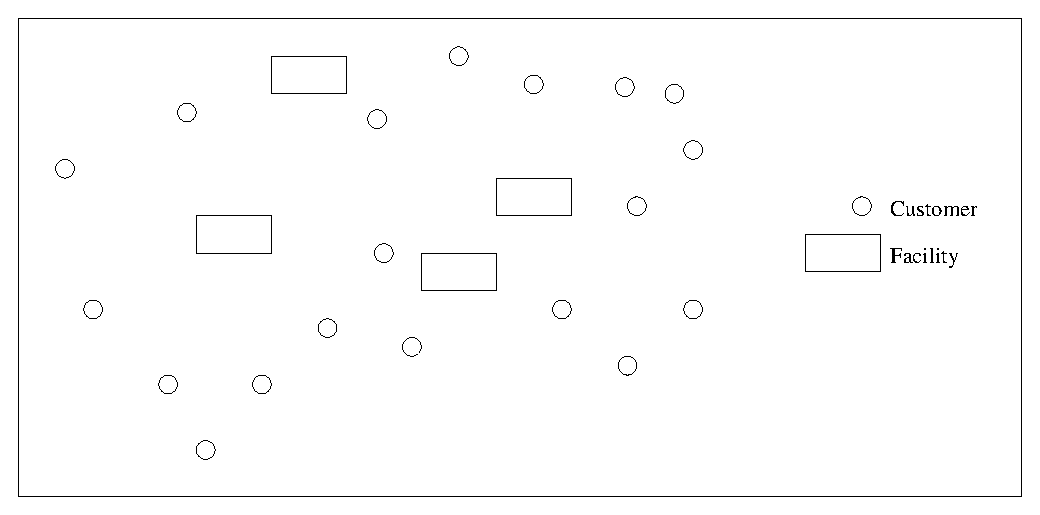
\includegraphics[scale=0.4]{lrsp-defn0}
}
%\subfigure[A solution to the instance]{
\subfigure[]{
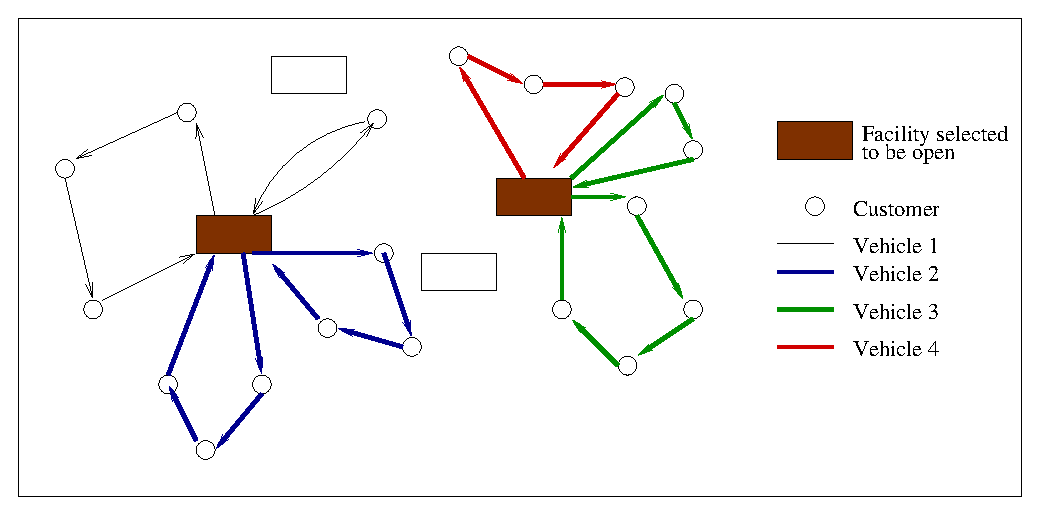
\includegraphics[scale=0.4]{lrsp-defn4}
}
\caption{\label{fig1a} Representation of the LRSP}
\end{center}
\end{figure}

The motivation behind the integration of the facility location, vehicle routing, 
and vehicle scheduling decisions is to improve the efficiency of the system and 
yield more cost-effective solutions. When it is possible to serve customers 
through routes making multiple stops, the cost of opening facilities can be captured
more accurately if we know the routing of the vehicles. This was realized  
as early as 1968; \citet{Webb} compared a cost function considering multiple stop tours
to a cost function based on straight line trips to customers in the context of 
determining the locations 
of depots with minimum cost. \citet{Salhi} also investigated the 
effect of ignoring the routing of vehicles while deciding the locations of facilities and showed 
that solving the location and routing problems independently does not always result in the best 
solution in terms of cost. Location and routing
problems (LRPs) seek to minimize total cost by simultaneously selecting a set
of facilities and constructing a set of delivery routes. LRPs, however, implicitly 
assume that each vehicle covers exactly one route. This may potentially overestimate 
the number of vehicles required and the associated distribution cost.
Therefore, considering the scheduling of vehicles while constructing the vehicle routes may result in a solution with a smaller number of vehicles that is a
better approximation of the real system. This is especially true when a 
vehicle may serve multiple routes and the problem has various scheduling
restrictions such as fleet size, different vehicle types, or time windows.
%Therefore, considering the scheduling of vehicles while constructing the vehicle 
%routes, especially when a vehicle may serve multiple routes and the problem has 
%various scheduling restrictions such as fleet size, different vehicle types, time 
%windows, may result in less number of vehicles and a solution which is a better 
%approximation of the real system.
Since the cost and environmental impact of logistics 
activities are quite high (total logistics costs only in U.S. were estimated to be
\$910 billion in 2002, equivalent to 8.7\% of GDP (\citet{MacroSys})), even a small 
amount of improvement in distribution systems can result in a substantial amount of 
savings. 
%As we describe, this research has made major economical, practical, theoretical  
%and computational contributions to the literature. 

In this paper, we provide mathematical programming models and describe 
exact and heuristic solution algorithms using branch-and-price methodology for an LRSP with 
capacity restrictions. Given a set of candidate facility locations and a set of customer locations, 
the objective of the problem is to select a subset of the facilities, 
construct a set of delivery routes, and assign routes to vehicles 
in such a way as to minimize total cost subject to satisfaction of the system's constraints.   
The main contributions of this paper are three-fold.  First, we present
two related formulations, one graph-based and one set-partitioning-based, for a version of the LRSP
in which there are capacity restrictions on both the facilities and vehicles as well as time restrictions
on the vehicles.  Second, we identify several classes of valid inequalities that can
strengthen the set-partitioning-based formulation and demonstrate their effectiveness empirically.
Third, we develop two versions of a branch-and-price algorithm that can provide optimal solutions 
for a variety of instances.

The remainder of the paper is organized as follows. Section~\ref{sec:models} provides a formal description
of the general LRSP and presents two formulations of the problem. Section~\ref{sec:algorithm} 
describes the components of the branch-and-price algorithm. Section~\ref{sec:results} 
presents results of the computational experiments. Section~\ref{sec:conclusion} concludes 
the paper and provides direction for future research.
 
\section{Literature Review}
The location routing and scheduling problem (LRSP) arises in the context of many 
delivery problems, such as gas, oil, food, beverage, bill and newspaper delivery problems. 
The LRSP generalizes and subsumes several well-studied problem 
classes, such as the vehicle routing problem (VRP) and the location routing problem (LRP). 
Vehicle routing models in general have been the subject of a wide range of
academic papers, but the number of these devoted to combined location and
routing models is much smaller. \citet{Laporte} surveyed the work on
deterministic LRPs and described different formulations of the problem,
solution methods used, and the computational results published up to 1988.
More recent review papers by \citet{Min} and \citet{Nagy} classify both 
deterministic and stochastic problems in the LRP literature with respect to 
problem characteristics and solution methods. 

Solution approaches for the LRP can be divided broadly into heuristics
and exact methods, with much of the literature devoted to heuristic
approaches. Most heuristic algorithms divide the problem into
subproblems and handle these subproblems sequentially or iteratively.
According to \citet{Min2}, for problems with large facility fixed costs and 
capacitated vehicles, sequential approaches perform computationally better. 
Examples of heuristics developed for the LRP can be found in
\citet{Perl}, \citet{Hansen}, \citet{Barreto07}, \citet{Srivastava},
\citet{Albareda-Sambola} and \citet{Prins}.

Exact algorithms for the LRP have been developed mostly for two-index vehicle flow 
formulations. \citet{Laporte81} solve a single depot model with a constraint relaxation 
method and a branch-and-bound algorithm. They report solving problems with 50 customer 
locations. \citet{Laporte83} solve a multi-depot model using a constraint relaxation 
method and Gomory cutting planes to satisfy integrality. They can solve problems with 
at most 40 customer sites. \citet{Laporte86} apply a branch-and-cut algorithm to a 
multi-depot LRP model with vehicle capacity constraints. They use subtour elimination 
constraints and chain barring constraints that guarantee that each route starts and 
ends at the same facility. The authors report computational results for problems with 20
customer locations and 8 depots. 

\citet{Belenguer06} provide two formulations of
the LRP with capacitated facilities and capacitated vehicles
using two-index variables. They 
present a set of valid inequalities for the problem and develop
two branch-and-cut algorithms based on the different formulations of the
problem. They report that they solve instances with up to
32 customers to optimality in less than 70 CPU seconds and provide
good lower bounds for the rest of the instances, which have up to 134
customers.

\citet{Berger} develops a set partitioning-based model for an LRP with route-length 
constraints and uncapacitated vehicles and facilities. \citet{Berger07} extend the work to 
develop an exact branch-and-price algorithm in which they solve the pricing problem as an
elementary shortest path problem with one resource constraint. They report computational 
results for problems with 100 customers and various distance constraints. 

As far as we know, the only LRSP papers in the literature to predate the 
earlier versions of this paper (\cite{Akca2} and \cite{Akca}) are \cite{Lin} 
and \cite{Lin2}, however, 
neither of them defined the class in full generality.
\cite{Lin} describe an application of the LRSP as
it arises in the delivery of telephone bills to housing projects in
Hong Kong.  They propose a heuristic approach in which they divide the problem into three
phases - facility location, vehicle routing, and vehicle assignment - 
and make multiple passes through each phase.  The authors test their algorithm
on generated instances including up to 12 customers and 4 facilities and on a
real instance with 27 customers and 4 facilities. 
\cite{Lin2} extend the heuristic algorithm of \cite{Lin} to 
solve instances of a multi-objective LRSP in which they seek to balance 
total cost, total vehicle time, and total vehicle load.  They test the algorithm on real 
instances with 27 and 89 customers and on generated instances with
100 and 200 customers.  Although \cite{Lin} report the development of a branch-and-bound
algorithm to solve instances of the LRSP exactly, neither \cite{Lin}
nor \cite{Lin2} provides a formulation of the problem.
\cite{Akca2} and \cite{Akca} describe the LRSP formally and develop formulations and solution algorithms; the full implementation is detailed in the 
remainder of the paper. More recently, \cite{Macedo14} describe an alternative network flow formulation and \cite{Macedo15} propose a meta-heuristic solution approach for the LRSP, a skewed Variable Neighborhood Search (VNS) algorithm. They present computational results for instances up to 100 customers. 


\section{Mathematical Programming Formulations}
\label{sec:models}
We consider an LRSP with capacity constraints
on the facilities and on the vehicles as well as time constraints on the vehicles.
In particular, given a set of candidate facility locations and a set of
customer locations, we seek a solution in which (i) each customer is visited exactly once, 
(ii) each route starts and ends at the same facility, (iii) the 
total demand of the customers assigned to a route is at most the vehicle 
capacity, (iv) the total working time of a vehicle is no more than the  
time limit, and (v) the total demand of the customers assigned to a facility 
does not exceed the capacity of the facility. 
The described problem is NP-hard.  To see this, consider an instance of the LRSP in which 
there is at most one vehicle
at each facility, there are no facility fixed costs, and the vehicle time limit is unrestricted.
Such a special case is equivalent to an instance of the MDVRP, which was shown to be
NP-hard by \cite{Bodin2} and \cite{Lenstra}.

We develop models for the delivery form of the LRSP and assume that there is no
service time at the customers.  The models, however, can be adapted easily for 
pickup problems and for nonzero service times.
At the heart of the LRSP is a network flow structure, deriving from the routing of customer demands,
that is constrained through the vehicle and facility capacities.  Hence, we consider both
arc-based and path-based formulations for the LRSP, as each has been widely applied
for related problems.
In Section \ref{sec:edge-based-form}, we present a three-index commodity flow 
formulation of the LRSP. In Section \ref{sec:set-part-form}, we present a 
set-partitioning-based formulation of the problem.  
In Section \ref{sec:StrongForm},
we introduce several classes of valid inequalities to strengthen the set-partitioning-based formulation.

\subsection{Graph-Based Formulation of LRSP}
\label{sec:edge-based-form}
%\rtbpapercomment{Needs an intro sentence}
For the related problems of LRP and VRP, the literature contains two main types of
graph-based models, vehicle flow and commodity flow. In both formulations, integer variables
represent the number of times a vehicle traverses a given arc or edge in an underlying
graph. In commodity flow formulations, there is an additional variable that represents the number of
units of a given commodity transported along the arc. In general, vehicle flow models 
contain an exponential number of subtour elimination constraints, 
whereas commodity flow models, with the help of additional flow variables, 
use a polynomial number of constraints to eliminate subtours. 
For the LRP and the VRP, two-index vehicle flow formulations are preferred 
in solution algorithms based on branch-and-cut since these formulations include 
a smaller number of variables and their LP relaxations yield better bounds. 
However, it is not possible to formulate the LRSP 
using variables with only two indices because of the time constraint for the vehicles. 
In this context, we require a three-index commodity flow model.
%\zelihaupdate{explain two index vs three index}

To formulate the model, we introduce the following notation.
Let $I$ be the set of customer locations and $J$ be the set of candidate facility locations.
We define a graph $G=(N,A)$ where $N=I \cup J$ is the set of nodes and 
$A= (J \times I) \cup (I \times I)$ is the set of arcs.   
Let $H_j$ be the set of vehicles, and let $\{H_j\}_{j \in J}$
be a partition of $H$ into  homogeneous sets of vehicles assigned to
each facility.
%all identical, located at facility $j$ such that  
%$H_{j_1} \cap H_{j_2} = \emptyset, \forall j_1, j_2 \in J$ and let $H=\cup_{j \in J}H_j$.


{\bf Parameters}
\begin{eqnarray*}
C^F_j & = & \mbox{daily equivalent fixed cost of opening facility $j$, $\forall j \in J$,} \\
C^O & = & \mbox{vehicle operating cost per unit travel time,} \\
C^V & = & \mbox{daily equivalent fixed cost of a vehicle (including the driver cost),} \\
D_i & = & \mbox{demand of customer $i$, $\forall i \in I$,} \\
L^F_j & = & \mbox{capacity of facility $j$, $\forall j \in J$,} \\
L^V & = & \mbox{capacity of a vehicle,} \\
L^T & = & \mbox{time limit for a vehicle and the driver, and} \\
T_{ij} & = & \mbox{travel time between locations $i$ and $j$, $\forall (i,j) \in A$.} 
\end{eqnarray*}

{\bf Decision Variables}
\begin{eqnarray*}
x_{ikh} & = & \left\{ \begin{array}{ll}
                 1  & \mbox{if vehicle $h$ travels on arc $(i,k)$, $\forall h \in H, (i,k) \in A$,} \\
                 0  & \mbox{otherwise,}                                                  
                \end{array} 
              \right. \\
y_{ikh} & = & \mbox{flow on arc $(i,k)$ carried by vehicle $h$, $\forall (i,k) \in A, h \in H$,} \\
t_{j} & = & \left\{ \begin{array}{ll}
                 1  & \mbox{if facility $j$ is selected, $\forall j \in J$,}\\
                 0  & \mbox{otherwise,}                                                  
                \end{array}  
              \right. \\
v_h & = &\left \{ \begin{array}{ll}
                 1  & \mbox{if vehicle $h$ is used, $\forall h \in H$, and}\\
                 0  & \mbox{otherwise.}                                                  
                \end{array}  \right. 
\end{eqnarray*}
{\bf (G-LRSP)} 
%{\bf Formulation}
\begin{optprog}
Min & \objective{\sum_{j \in J} C^F_j t_{j}  + C^V \sum_{h \in H} v_h  + C^O \sum_{h \in H} \sum_{(i,k) \in A}T_{ik} x_{ikh} } \label{obj-eb} \\
s.t. & \sum_{h\in H}\sum_{k \in N} x_{ikh} & = & 1 &  \forall  i \in I, \label{set-part}\\
           & \sum_{k\in N} x_{ikh}-\sum_{k \in N} x_{kih} & = & 0 & \forall i \in N, h \in H, \label{enterleave}\\
           & \sum_{h \in H_j}\sum_{k \in I} y_{jkh} - L^F_j t_{j} & \leq & 0 & 
	   \forall j \in J, \label{FacCap}\\
           & y_{ikh} - L^V x_{ikh} & \leq & 0 & \forall (i,k) \in A, h \in H, \label{VehCap}\\
           & \sum_{k \in I} y_{ikh} - \sum_{k \in I} y_{kih} + D_i\sum_{k \in N}x_{ikh} & = & 0 & \forall i \in I, h \in H, \label{flow-conv}\\
           & \sum_{(i,k) \in A} T_{ik} x_{ikh} - L^T v_h & \leq & 0 & \forall h \in H, \label{timeLim}\\
          % & \mbox{NumH} - \sum_{h \in H} \mbox{Dri}_h & = & 0 & \\
           %& \mbox{Tot} - \sum_{h \in H}\left[\sum_{i \in I}\sum_{k \in I}\left(t_{ik}+s_{k}\right)x_{ikh}\right] / 60 & = & 0 & \\
         %  & x_{jih} - T_{j} & \leq & 0 & \forall j \in M, i \in I, h \in H \label{Rel-X-T-1}\\
 %          & x_{ijh} - T_{j} & \leq & 0 & \forall j \in M ,i \in I, h \in H \label{Rel-X-T-2}\\
         %  & x_{jkh} & = & 0 & \forall j \in J,k \in N, h \in H_t, t \in J \backslash \{j\},\label{fix-0} \\ 
           & x_{jkh} & = & 0 & \forall j \in J,k \in N, h \in H_t,  \nonumber \\
           & & & & t \in J \backslash \{j\},\label{fix-0} \\
           & x_{ikh} & \in & \{0,1\} & \forall (i,k) \in A, h \in H, \label{x-var}\\
           & y_{ikh} & \geq &  0 & \forall (i,k) \in A, h \in H, \label{y-var} \\           
           & t_{j}  & \in & \{0,1\} & \forall j \in J, \mbox{ and} \label{t-var}\\
           & v_{h} & \in & \{0,1\} &  \forall h \in H. \label{dri-var}
        %  & \mbox{Tot} & \geq & 0 
\end{optprog}

The objective function (\ref{obj-eb}) states that the total cost, which  
includes the fixed cost of the selected facilities, the fixed cost of the vehicles
(including the driver cost), and the operating cost of the vehicles,
should be minimized. 
%The objective function (\ref{obj-eb}) seeks to minimize the total cost, which  
%includes the fixed cost of the selected facilities, the fixed cost of the vehicles
%(including the driver cost), and the operating cost of the vehicles. 
Constraints 
(\ref{set-part}) specify that exactly one vehicle must travel from customer node $i$
to some other node. Constraints (\ref{enterleave}) require that a vehicle should enter 
and leave a node an equal number of times. For customer nodes, constraints 
(\ref{set-part}) and (\ref{enterleave}) ensure that if a vehicle enters a 
customer node, it will leave this node and therefore that each customer 
node is served exactly once. For facility nodes, the number of visits by any 
vehicle can exceed one, since a vehicle can cover multiple routes. 
Constraints (\ref{FacCap}) ensure that the total outbound flows to the customer nodes 
from each facility do not exceed its capacity. 
Constraints (\ref{VehCap}) are vehicle capacity constraints and define the 
relationship between the binary variable $x_{ikh}$ and the flow variable 
$y_{ikh}$. Each constraint ensures that flow between any pair of nodes
cannot exceed the capacity of a vehicle. Constraints (\ref{flow-conv})
require conservation of flow at each customer node; these constraints
must be modified for pick-up problems.
Constraints (\ref{VehCap}) and (\ref{flow-conv}) 
together ensure that no route violates the vehicle capacity.
The combined sets of constraints (\ref{set-part}), (\ref{enterleave}),
and (\ref{flow-conv}) ensure that only valid traveling salesman
tours that include a  facility are formed, as in 
\citet {Nambiar}.  Constraints (\ref{timeLim}) limit the 
total time of a vehicle's schedule to the time limit. 
Constraints (\ref{fix-0}) restrict travel on the arcs originating from 
a facility to vehicles located at that facility.
Constraints (\ref{x-var}), (\ref{y-var}), (\ref{t-var}), and (\ref{dri-var}) 
are the integrality and non-negativity requirements on the variables.    

%\zelihaupdate{Complexity sentences does not belong here!}


G-LRSP is a three-index commodity flow formulation.
Because of the facility and vehicle capacity restrictions, we cannot
know a priori the number of vehicles required at each facility, though the
number is clearly at most $|I|$.  Thus, this formulation can require
up to $O(|I|^4)$ binary variables 
and $O(|I|^4)$ constraints, which can be as many as 6 million for an 
instance with $50$ customers. 
%\zelihaupdate{rewrite ..} 
Although it would be possible to develop 
a branch-and-bound algorithm for G-LRSP, %formulation, 
we suspect
that such an approach would not yield positive results, given the inherent
symmetry in the formulation and the known difficulty 
associated with solving related problems.
% with three-index formulations.  For example, there are no exact
%algorithms based on three-index vehicle or commodity flow formulations of the LRP. 
%In addition, G-LRSP includes a large amount of symmetry under the assumption
%of identical vehicles, which makes the solution difficult. 
Instead, we propose a set-partitioning-based formulation 
similar to those that have been successful for other hard combinatorial problems.


\subsection{Set-Partitioning-Based Formulation of LRSP}
\label{sec:set-part-form}
In this section, we introduce a set-partitioning-based formulation of 
the LRSP. The set-partitioning-based formulation (SPP-LRSP) presented here is 
equivalent to the model obtained by applying Dantzig-Wolfe decomposition (DWD)
to G-LRSP (for details, see \cite{Akca}), though it was not developed 
using that technique.  
In the application of the DWD  method, constraints (\ref{set-part})
and (\ref{FacCap}) form the master problem, while the remaining constraints 
define the subproblem. This subproblem then can be decomposed by facility
and further by vehicle. 
The equivalence of SPP-LRSP and the DWD of G-LRSP follows after a further
reduction in the subproblem column set based on symmetry and 
constraints in the master problem.
%The equivalence of the SPP-LRSP and the DWD of the 
%G-LRSP follows after a further reduction in the resulting set of columns based 
%on symmetry and constraints in the master problem.   

To define the column set, the set-partitioning-based formulation uses the idea of a 
{\em pairing}, which we adapt from the pairing concept in the crew scheduling literature 
(e.g., \citet{Desrosiers}, \citet{Vance}, and \citet{Anbil}). In the 
crew scheduling literature, a pairing is a sequence of duty periods 
and represents  a possible schedule for a single crew. In the LRSP context, 
a pairing is a sequence of routes that represents a possible (feasible) schedule for a 
single vehicle. In other words, as explained below, pairings are defined by the subproblem constraints
in the DWD of G-LRSP, i.e., constraints  (\ref{enterleave}), (\ref{VehCap}),
(\ref{flow-conv}), (\ref{timeLim}), (\ref{fix-0}), (\ref{x-var}), (\ref{y-var}), (\ref{t-var}), 
and (\ref{dri-var}), decomposed by vehicle. 

A pairing is feasible if (i) each route included in the pairing starts and ends at the 
same facility, (ii) for each route in the pairing, the total demand of the 
customers assigned to the route is at most the vehicle capacity, and (iii) the total travel 
time of the pairing is at most the vehicle time limit. 
In addition to these constraints, we require that (iv) each
customer included in the pairing be visited only once. 
By adding constraint (iv), we prevent the generation of pairings that
visit some customer(s) multiple times since such pairings are set 
to zero in an integer feasible solution of an LRSP.

Figure \ref {fig:exppair} shows two possible pairing constructions.  
Pairing 1 includes routes 1, 2 and 3; pairing 2 includes routes 4 and 5. 
Each pairing specifies the routes covered by a vehicle and has an associated  
cost, which is defined as the sum of the costs of the component routes plus a
fixed cost for the vehicle. Since the cost of a multiple-stop route depends on the sequence 
of nodes visited, the pairing information implicitly includes sequencing information
for each route. The cost of a pairing, however, is not affected by the ordering of
the routes in the absence of time windows and thus is arbitrary.  We will take this
fact into consideration in the solution of the subproblem and will not generate symmetric
pairings corresponding to different orderings of the same routes.

%Even though the set of routes in a pairing may be 
%ordered in principle, the ordering 
%of the routes does not affect cost in the absence of time windows and is thus arbitrary. We will consider this fact in 
%the solution of the subproblem and will not generate symmetric pairings corresponding
%to different orderings of the routes. 

\begin{figure}[h]
  \centering
  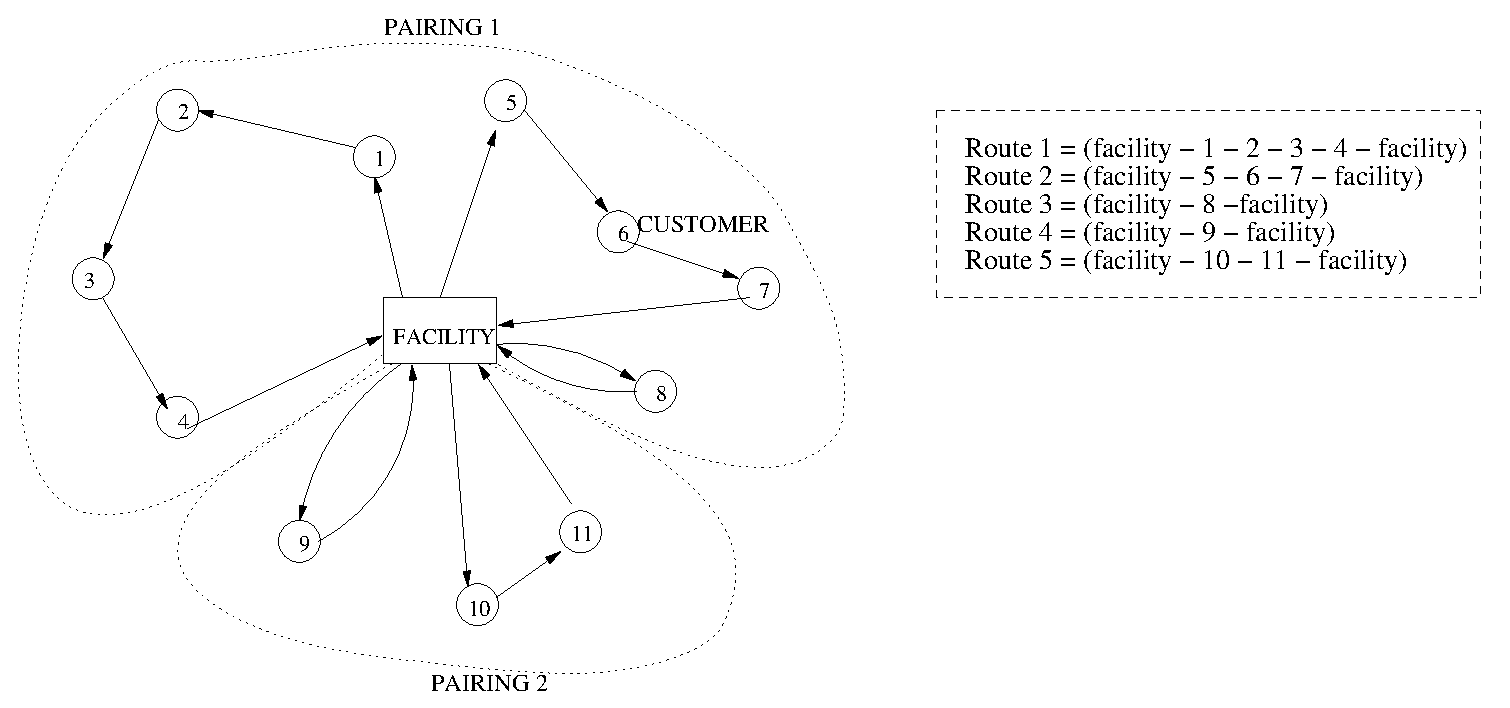
\includegraphics[scale=0.5]{./pairexp2}
  %\fbox{ \includegraphics[scale=0.5]{figure/pair2.eps}}
  \caption{Example of pairings} \label{fig:exppair}
\end{figure}

Given a set of candidate facility locations and the set of feasible pairings that can 
be constructed for each candidate facility, the objective of the LRSP is to select a 
subset of the facilities and an associated subset of pairings in such a way 
as to minimize the total cost subject to the following constraints: (i) each 
customer must be covered by exactly one pairing, (ii) the total demand of the 
customers assigned to a facility must not exceed the capacity of the facility, 
and (iii) vehicles cannot be associated with a facility unless it is open. 

To present the formulation, we define additional parameters and 
decision variables.  Associated with each candidate facility 
$j \in J$, we let $P_j$ be the set of all feasible pairings for facility
$j$.   

{\bf Parameters}
\begin{eqnarray*}
a_{ip} & = & \left \{  \begin{array}{ll}
                 1 & \mbox{if customer $i$ is in pairing $p$ of facility $j$, $\forall i \in I, p \in P_j, j \in J$,} \\
                 0 & \mbox{otherwise, and}
                         \end{array}
              \right. \\
C_p & = & \mbox{cost (vehicle fixed cost plus operating cost) of pairing $p$ %associated with 
of facility $j$,}\\
& &  \mbox{$\forall p \in P_j, j \in J$.} 
%L^F_j & = & \mbox{capacity of facility $j$, $\forall j \in J$} 
\end{eqnarray*}

{\bf Decision Variables}
\begin{eqnarray*}
t_j &  = & \left \{ \begin{array}{ll}
                 1  & \mbox{if facility $j$ is selected, $\forall j \in J$,}\\
                 0  & \mbox{otherwise,}                                                  
                \end{array}
       \right. \\
z_p & = & \left \{ \begin{array}{ll}
                 1  & \mbox{if pairing $p$ is selected for facility $j$, $\forall p \in P_{j}, j \in J$, and}\\
                 0  & \mbox{otherwise.}                                                  
                \end{array}
       \right.
\end{eqnarray*}
{\bf(SPP-LRSP)} 
%{\bf Formulation}
\begin{optprog}
Min & \objective{\sum_{j \in J} C^F_j t_{j} + \sum_{j \in J} \sum_{p\in P_j} C_p z_p} \label{spp-obj}\\
subject to & \sum_{j \in J} \sum_{p \in P_{j}} a_{ip} z_{p} & = & 1 & \forall i \in I, \label{spp_con1} \\
           & \sum_{p \in P_j} \sum_{i \in I} a_{ip} D_i z_{p} - L^F_j t_j & \leq & 0 & \forall j \in J, \label{spp_con2} \\
           & t_{j}  & \in & \{0,1\} & \forall  j \in J, \mbox{ and}\label{binary1} \\
           & z_{p} &  \in & \{0,1\} & \forall p \in P_j, j \in J. \label{binary2} 
\end{optprog} 
 
The objective function (\ref{spp-obj}) seeks to minimize the total cost.
%, which includes the fixed cost of the selected facilities and the cost of the selected pairings. 
Constraints (\ref{spp_con1}) 
%guarantee that each customer location is served by exactly one pairing. 
states that each customer must be in exactly one of the selected pairings.
Constraints (\ref{spp_con2}) 
guarantee that the total demand of the customers assigned to
a facility does not exceed the facility capacity.  
%Constraints (\ref{spp_con2}) 
%ensure that the total demand of the selected pairings does not exceed the facility capacity.  
Constraints (\ref{binary1}) and (\ref{binary2}) are standard binary restrictions on the 
variables. 

The SPP-LRSP formulation eliminates the symmetry that arises in G-LRSP because of the
identical vehicles; here we enumerate one set of feasible pairings that can be assigned to any vehicle 
located at a facility instead of duplicating this set for each vehicle located at a facility. 
Furthermore, the pairing concept removes the symmetry caused by the different orderings of routes in a 
vehicle's schedule since the ordering is arbitrary.

\subsection{Strengthening the Set-Partitioning-Based Formulation}
\label{sec:StrongForm}
In this section, we discuss how we can strengthen the set-partitioning-based formulation
SPP-LRSP by adding valid inequalities. First, we introduce a lower bound on the total 
number of facilities required in any integer feasible solution.  Let $R$ denote a lower bound
on the minimum number of required facilities. 
Then we can add to SPP-LRSP a constraint to force the number of selected
facilities to be at least $R$:
\begin{eqnarray}
\sum_{j \in J} t_{j} \geq R. \label{lb-open-fac}
\end{eqnarray}
For any instance, we can calculate a valid value for $R$ from the demands of the customers and
the capacities of the facilities.  If all of the facilities have the same capacity value,
$L^F_j = k$ $\forall j \in J$, then 
\begin{equation}
R =\left \lceil \frac{\sum_{i \in I} D_i}{k} \right \rceil . \nonumber
\end{equation}
%\item 
If at least one facility capacity differs, then a lower bound on the number of required
facilities can be calculated using a greedy algorithm: compute the total demand and assign
it to the facilities in non-increasing order of their capacities.  Let $n = |J|$ and 
let $(j_1,j_2,..,j_n)$ be an ordering of the facilities such that 
$L^F_{j_1}\geq L^F_{j_2} \geq ...\geq L^F_{j_n}$. Then,
\begin{eqnarray}
 R = \mbox{argmin}_{\{l = 1..n\}} \left (\sum_{t=1}^{l}L^F_{j_t}\geq \sum_{i \in I} D_i \right ).  
\end{eqnarray}
%\end{itemize}
Constraint (\ref{lb-open-fac}) is not necessary in the formulation of the LRSP. However, as a simple
lower bound on the number of required facilities, it may eliminate some solutions in which 
a fractional number of facilities is used, thereby improving the LP relaxation bound.
\cite{Akca} shows that constraint (\ref{lb-open-fac}) has a Chv\'atal-Gomory (CG) rank
of one under certain conditions.

We introduce a second set of constraints by linking the facility variables and the pairing
variables.  For the capacitated facility location problem (CFLP), 
\cite{Leung} show that the constraints that link the facility variables and 
the assignment variables are facets 
of the CFLP polytope if the demands of the customers are less than the capacities of the facilities.  
\citet{Daskin} shows that these constraints improve the LP relaxation bound considerably.  
Due to the similarity in structure between
the CFLP and SPP-LRSP, we consider adding the constraints
\begin{eqnarray}
t_{j} - z_{p} \geq & 0  & \forall j \in J, p \in P_{j}. \label{relation-Z-T}
\end{eqnarray}
These constraints ensure that a pairing is selected only if its associated facility is open.  
Constraints (\ref{relation-Z-T})
are implied by constraints (\ref{spp_con2}) and the integrality constraints, but their addition 
may improve the LP relaxation bound, as in the case
of the CFLP.  However, having one constraint associated with each pairing is 
undesirable in a set-partitioning-based formulation with an exponentially large
number of columns.   
%In addition, it is not clear how to associate
%constraints (\ref{relation-Z-T}) with the pricing problem. 
We consider instead the following set of inequalities, which are valid for the integer program:
\begin{eqnarray}
    t_j - \sum_{p \in P_{j}}a_{ip}z_{p}\ \geq \ 0 \mbox{\ \ $\forall j \in J$, $i \in I$.} \label{relation}
\end{eqnarray}
Note that these are similar to the inequalities developed by \cite{Berger07}.
In a feasible integer solution, each customer $i \in I$ is served by exactly one pairing, so $\sum_{p \in P_j}
a_{ip} z_{p}$ is 1 for some facility $j$ and 0 for all others.  For any facility such that $\sum_{p \in P_j}
a_{ip} z_{p}$ is 1, $t_j$ will be 1, which corresponds to selecting only pairings associated with open facilities.


% It is difficult to say something about the relationship between this constraint and constraint (14).
% In general Constraint (14) implies these constraints. If total demand d(N) <= FCap, then
% we can omit (14) and just use these (multiply each with D_i and sum. It will be equal or stronger than
% (14) Feasible region with these is smaller than the region with (14) since these are disaggregated constraints
% but (14) is aggregated. However, if d(N)> FCap, then the feasible region comparison can not be done since
% summation of these constraints are weaker than (14).  

%[INSERT: do these imply (14)? are they implied by (14)?  Can we say anything about the corresponding feasible region??]

In Section \ref{sec:results}, we demonstrate empirically the improvement in the LP relaxation 
bound of the SPP-LRSP formulation that results from adding constraints (\ref{lb-open-fac}), 
(\ref{relation-Z-T}), and (\ref{relation}). 
As we will show, adding both constraints (\ref{lb-open-fac}) and (\ref{relation}) to 
SPP-LRSP yields the largest improvement.  Throughout the remainder of the paper, we use
an augmented SPP-LRSP formulation, denoted AUG-SPP-LRSP, which is comprised of the 
objective function (\ref{spp-obj}) and constraints (\ref{spp_con1}), 
(\ref{spp_con2}), (\ref{binary1}), (\ref{binary2}), (\ref{lb-open-fac}), and (\ref{relation}). 

\section{Solution Algorithm} 
\label{sec:algorithm}
In our set-partitioning-based formulation of the LRSP, each column corresponds to a feasible
pairing.  For medium- and large-sized instances, the number of feasible pairings can be 
extremely large, making it unlikely that we can efficiently solve instances that 
explicitly include all feasible pairings. Instead, we have developed a branch-and-price
algorithm in which we dynamically generate only a subset of the feasible pairings
at each node of the tree.

Branch and price has become a standard approach for solving large-scale integer programming
problems, especially those formulated using set-partitioning-based models. 
\citet{Barnhart} discuss the general methodology and the many  
challenges in developing a branch-and-price algorithm. 
The algorithm has been applied to a variety of problems, including various vehicle routing problems 
(\citet{Fukusawa}),
location routing problems (\citet{Berger07}, \citet{Akca3}) and  
airline crew scheduling problems (\citet{Vance}), all of which are relevant in the context of the LRSP.

In the following sections, we describe the components of the branch-and-price algorithm
that we developed for the LRSP.
In Section \ref{sec:PricingProb}, we describe the column generation algorithm for solving
the LPs at the nodes of the branch-and-price tree. In Section \ref{sec:BranchingRules}, 
we describe the branching rules. In Section \ref{sec:BPAlgorithm}, 
we present implementation details of the algorithm. 

\subsection {Column Generation}
\label{sec:PricingProb}
Column generation is an approach for solving LPs for which we want to avoid explicitly enumerating
all columns.  The basic idea is to determine a subset of the variables that includes 
those that are nonzero in some optimal solution. By solving the LP including only this subset of 
columns rather than all possible columns, we can obtain the optimal LP solution. 
%Thus, to avoid generating all possible feasible pairings, we use column generation. 
Here, we explain the terminology and the main steps of the column generation within the branch-and-price
algorithm developed for the LRSP.  

In each iteration of our column generation procedure, we work with a restricted version of the LP relaxation; this
{\em restricted master problem} (RMP) includes all of the facility location variables but
only a subset of the pairing variables.  We solve the RMP and use the associated dual variable
information to formulate the {\em pricing problem}.  The objective
of the pricing problem is to either identify new columns to add to the RMP or prove 
optimality of the current solution. From the theory of linear programming, we know that 
if every variable has a non-negative reduced cost, then the solution is optimal.  Therefore, 
in the context of the LRSP, the objective
of the pricing problem is to determine if there are feasible {\em pairings} with negative reduced
cost that can be added to the RMP.  If the pricing problem identifies at least one pairing with 
negative reduced cost, then we add one or more 
columns to the RMP and reoptimize.  Otherwise, the current solution is optimal for the full problem.

As explained in Section \ref{sec:set-part-form}, we decompose the pricing problem
into a set of independent pricing problems, one for each facility. 
%The constraints of the pricing problem are listed in Section \ref{sec:set-part-form}.  
To write the objective function for facility $j$, 
we consider formulation AUG-SPP-LRSP and obtain an expression for the reduced
cost of a pairing.  
 Let $\pi_{i}$ be the dual variable 
associated with constraint (\ref{spp_con1}) for customer $i$, $\mu_{j}$ be 
the dual variable associated with constraint (\ref{spp_con2}) 
for facility $j$, and $\sigma_{ji}$ be the dual variable for linking 
constraint (\ref{relation}) for facility $j$ and customer $i$. 
For the variable $z_{p}$ for $p \in P_{j}$, the reduced cost $\hat{C}_{p}$
can be written as   
\begin{eqnarray}
\label{red-cost}
\hat{C}_{p}=C_{p}-\sum_{i\in I}a_{ip} \pi_{i}+\sum_{i \in I}a_{ip} D_{i} \mu_{j}+\sum_{i \in I} a_{ip} \sigma_{ji},
\end{eqnarray} 
where $C_{p}$ is the cost of pairing $p$. 
Then, we can express the pricing problem for facility $j$ as the problem of 
minimizing $\hat{C}_p$ subject to the appropriately indexed constraints 
from (\ref{enterleave}), (\ref{VehCap}),
(\ref{flow-conv}), (\ref{timeLim}), (\ref{fix-0}), (\ref{x-var}), (\ref{y-var}), (\ref{t-var}), 
and (\ref{dri-var}).

One approach to solving the pricing problem is to formulate it as a network problem. 
\cite{Akca2} describes the details of such a network problem, which is 
a modified elementary shortest path problem with resource constraints (ESPPRC). 
An alternative approach is to extend the first approach to a two-phase pricing problem: first generate a set of feasible 
vehicle routes and then combine them to construct a feasible pairing of minimum reduced cost. 
Each phase is also formulated as a network problem and solved as an ESPPRC. Since the 
two-phase approach showed better performance in our experiments, we describe the details here.

\subsubsection{Two-Phase Pricing Problem}
%The overall objective of the two-phase approach is to identify a feasible pairing with negative reduced
%cost, if there is one. 
Since a pairing is a set of routes, we can express the variable
 part of the reduced cost of a pairing 
%((\ref{red-cost}) minus the vehicle fixed cost
%that is included in the term $C_p$) 
as the sum of the reduced costs of the routes 
forming the pairing. For there to exist a negative reduced cost pairing 
composed of more than one route, there must exist negative reduced cost routes.
Otherwise, the pairing including only the single route with the lowest reduced
cost would be the lowest cost pairing overall.  
Thus, the basic idea of the
two-phase approach is to generate feasible routes first. 
If there are negative reduced cost routes, then combine these routes to generate 
pairings with more negative reduced cost.  Otherwise, update the reduced 
cost of the first-phase routes with the fixed cost to obtain a column (a single-route pairing) with negative 
reduced cost or to conclude that the current solution is optimal.  

\paragraph{Phase One: Generating Routes}
From the constraints of the pricing problem, a route is feasible 
if it starts and ends at the same facility, 
visits a customer at most once, and satisfies the vehicle capacity and the
vehicle time limit constraints. 
To generate feasible routes, we construct a network with $|I| + 2$ nodes: 
one node for each of the $|I|$ customers, one node for the facility as a {\em source} and one node
for the facility as a {\em sink}.  Each customer node has a demand equal to its demand in the original
problem.  The network includes an arc from the source to each customer node, a pair of directed arcs 
between each pair of customer nodes, and an arc from each customer node to the sink node. 
In the constructed network, an elementary path  feasible with respect to 
two resource constraints (vehicle capacity and time limit) corresponds to a feasible vehicle route.  
In order to minimize the reduced cost (\ref{red-cost}), the cost of each link in the network
for facility $j$ is modified with associated dual variables: 
% The cost of each arc
%is the {\em reduced cost} of the arc.  To obtain the reduced cost, we transfer the dual variables 
%$\pi_i$, $\mu_j$ and $\sigma_{ji}$ associated with the nodes to the appropriate arcs, 
%in particular, to the arcs entering the customer node $i$. The cost function for the pricing problem
%for facility $j$ is  
\begin{equation}
\hat{c}_{ki}   =  \left \{ \begin{array}{ll}
                 c_{ki} - \pi_i + D_{i} \mu_{j}+\sigma_{ji} \ \ & \mbox{if $i \in I$,}\\
                 c_{ki}  & \mbox{otherwise,}                                                  
                \end{array}
       \right. 
\end{equation}
where $c_{ki}$ is the operating cost of the link $(k, i)$.  
%In particular, we transfer the dual variables associated with node $i$ to all of the arcs entering node $i$.
Then, the cost of a path in the network is equal to the reduced cost of the corresponding route.
To determine if there is a feasible route with negative reduced cost, we solve an elementary shortest path
problem with two resource constraints (vehicle capacity and time) by applying the
extended label correcting algorithm of \citet{Feillet}.

In the \citet{Feillet} algorithm, each path from the source to a node in the network is assigned a 
{\em label}, which is a vector of the reduced cost of that (partial) path, the resources consumed (vehicle 
load and elapsed time),
the customer nodes included in the path, and the customer nodes that cannot  
be visited due to the resource constraints.  Customers are considered {\em unreachable} if
they have already been visited in the path or if they cannot be served by the vehicle without
violating a resource constraint. The algorithm fans out from the source node,
repeatedly examining the nodes of the graph.  Each time it examines a node, the algorithm 
extends each of the paths to each possible successor node, continuing until no further extensions are feasible.  

To reduce the set of labels to be extended, the algorithm
includes domination rules that compare the reduced cost, the time, the vehicle capacity, 
and the set of unreachable customers.  
To be more specific, let $l_1$ and $l_2$ be two labels for a node.  Label $l_1$ dominates label $l_2$
if all of the following conditions are satisfied: (i) the current travel time and the vehicle load 
of $l_1$ are less than or equal to those of $l_2$, 
(ii) the reduced cost of $l_1$ is less than or equal to the reduced cost of $l_2$, and 
(iii) for all nodes $i \in I$, $i$ is reachable only in label $l_1$ or $i$ is 
unreachable in both labels  $l_1$ and  $l_2$.
The algorithm stores and extends only non-dominated labels
at each node.  At the end of the algorithm, each label at the sink node corresponds to 
a feasible vehicle route with an associated reduced cost.  

Let $S$ denote the set of feasible routes with negative reduced cost at the
sink. If $S$ is non-empty, we continue with phase two. Otherwise, we add the
fixed cost from expression (\ref{red-cost}) to the cost of the smallest
reduced cost route to obtain the reduced cost of that single-route pairing.
If this reduced cost is zero or positive, then we
can conclude that the current LP relaxation solution is optimal. Otherwise,
we have a pairing with negative reduced cost to add to the RMP.
Note the implication that, even in the case where there are no
\emph{routes} with negative reduced cost, we may still get a negative reduced
cost \emph{pairing} (consisting of a single route) when the fixed cost
associated with the vehicle is negative. This can occur after applying certain
branching rules (see Section \ref{sec:BranchingRules}).

%However, as we explain in Section \ref{sec:BranchingRules}, one of our branching rules results
%in adding a fixed cost that may be negative to the reduced cost expression. Even in this case, however, 
%we do not proceed to phase two when the set $S$ is empty, since pairings including single routes
%will still have lower reduced costs since combination of positive reduced cost routes results 
%in larger reduced cost.   

\paragraph{Phase Two: Generating Pairings}
The objective of phase two is to generate feasible negative reduced cost pairings
by combining the routes in set $S$.
Two (or more) vehicle routes can be combined to form a feasible pairing if they do not have
customer nodes in common and they can both (all) be completed within the vehicle's time limit.
Finding a feasible pairing with the minimum reduced cost again corresponds to solving a
resource constrained elementary shortest path problem.

We construct a network
with $2 + |S|$ nodes: a source node, a sink node and one ``intermediate'' node 
to represent each of the vehicle routes in set $S$.  The network includes an arc from the source node to 
each intermediate node, arcs between pairs of intermediate nodes, and an arc from each intermediate node 
to the sink node.  Note that, because the sequence of routes in a pairing
is arbitrary, we only include an arc from an intermediate node to another intermediate node with higher
index.  Associated with each arc inbound to an intermediate node are two values: the time required to
complete the corresponding route and the reduced cost of the route.  The time and cost for arcs inbound
to the sink are zero.  To find a feasible pairing with the minimum reduced cost, we solve an ESPPRC
with a single resource constraint (time).  As in phase one, we apply
the extended label correcting algorithm of \cite{Feillet}.  At the end of the algorithm, 
each label at the sink node corresponds to a feasible pairing with an associated {\em negative} 
reduced cost. The costs of pairings at the sink node are updated with the fixed cost
that must be included in the reduced cost of a variable, and any pairing with 
negative reduced cost is a candidate pairing to add to the RMP.
Since we solve the exact ESPPRC algorithm in each phase of the  algorithm, the 
overall pricing algorithm is exact and results in a column with the most negative reduced cost, if any. 
In the remainder of the paper, we refer to this exact pricing algorithm as 2p-ESPPRC.

\subsubsection{Heuristic Pricing Algorithms}
The two-phase approach (2p-ESPPRC) is an {\em exact} algorithm in that it is guaranteed to generate a column
with the minimum reduced cost.  The downside of the approach is that it may not be
very efficient for large problems.  To find feasible solutions (pairings) more quickly, we define 
two heuristic versions of the algorithm.  The first heuristic restricts the state space 
of the exact algorithm by directly restricting the number of labels (proposed
by \citet{Dumitrescu}). In particular, during 
either phase of the algorithm, we can limit the maximum number of 
labels at each node that are stored to be extended.  During the algorithm,
as we update the list of labels, we order the labels in increasing order of reduced cost 
and we keep at most the first {\em label limit} number of non-processed  labels.  
We refer to this heuristic pricing algorithm as 2p-ESPPRC-LL(n), where n is the value
of the label limit.

The second heuristic restricts the state space by considering just a subset of the 
customers instead of all of them. In this way, the total number of labels to be 
generated is restricted indirectly. In each pricing iteration for a facility,   
we determine two customers that have the lowest reduced costs from the facility.  
We initialize the subset with these two
customers since we expect to have at least two routes in a pairing.  Then, by 
exploring the links from the subset of customers to the remaining customers, we repeatedly add one customer 
that is connected by a cheapest link to the subset until 
the size of the subset is equal to the determined {\em subset size}.
The 2p-ESPPRC is run for the selected subset of customers. 
We refer to this algorithm as 2p-ESPPRC-CS(n), where n is the subset size.

%If a heuristic version of phase one identifies routes with negative reduced cost, the routes are valid
%and can be used to generate pairings in phase two.  If the heuristic version of phase two identifies
%pairings with negative reduced cost, they are valid and may be added to the RMP.
If the heuristic versions of the pricing algorithm,  2p-ESPPRC-LL(n) and 2p-ESPPRC-CS(n),
do not identify any columns with negative reduced cost, the exact version  2p-ESPPRC 
must be applied in order to conclude whether or not there exist columns with negative reduced cost.  

\subsection {Branching Rules}    
\label{sec:BranchingRules}
An important step in developing a branch-and-price algorithm is devising good branching rules.
Branching rules that affect the structure of the pricing problem may make column generation
 more difficult.  Therefore, the main 
objective is to find disjunctions that eliminate as much of the integer infeasible region 
as possible but that minimize the increase in difficulty of solving the pricing problem. We apply four 
branching rules in our branch-and-price algorithm. 

First, we apply standard variable dichotomy branching for the facility location variables $t$. 
For a fractional variable $t_j$, in the right branch, we set $t_j = 1$, which forces facility location 
$j$ to be open. The pricing problem for the right branch does not change since $t$ variables
are not present in the constraints of the pricing problem, and the pricing problem for each facility
is independent from the others.  In the left branch, we set   
$t_j = 0$, which forces facility location $j$ to be closed.  Since
the facility is closed, no pairings associated with the facility are allowed in the solution, so there
is no need to solve the pricing problem. In addition, we set all $z_{p}$ variables for facility $j$
to 0.

Second, we consider the total number of vehicles at each facility. By definition, a pairing is associated
with a single facility and corresponds to one vehicle.  Thus, in 
any integer solution, the number of vehicles (pairings) used at any facility must be integer. 
Let $w_j$ be the number of vehicles used at facility $j$.  Then,  
\begin{eqnarray}
  \label{n-equal}
  w_j =\sum_{p \in P_j} z_{p} \qquad \forall j \in J. 
\end{eqnarray}    
If we add the equalities (\ref{n-equal}) to the master problem, we can branch explicitly on
the $w_j$ variables. Assume that in a fractional solution $w_j=b$, where $b$ is not integer.
In one branch, we require $w_j\geq \lceil b \rceil$; in the other
branch, we require  $w_j\leq \lfloor b \rfloor$.
Branching on the $w_j$ variables instead of implicitly  branching
on $\sum_{p \in P_j}z_{p}$ is an example of explicit constraint branching, an idea developed by 
\citet{Appleget} to improve the performance of branch-and-bound algorithms for mixed integer
linear problems. These new variables make it easier to identify the necessary 
updates to the pricing problem. 
Let $\beta_j$ be the dual variable associated with constraint (\ref{n-equal}) for facility $j$.
Then, the reduced cost of the variable $z_{p}$  changes to the following:
\begin{eqnarray}
  \label{new-red-cost}
  \hat{C}_{p}=C_{p}-\sum_{i\in N}a_{ip} \pi_{i}+\sum_{i \in N}a_{ip} D_{i} \mu_{j}+\sum_{i \in N}a_{ip} \sigma_{ji}-\beta_j
\end{eqnarray} 
In equation (\ref{new-red-cost}), we can interpret $\beta_j$ as a fixed cost for facility $j$ that is
independent of pairing $p$ and the included customers.  Therefore, we do not need 
to change our network structure or the pricing problem structure to incorporate $\beta_j$. 
Instead, we can calculate the cost of a path in the modified network in the same way as before and 
then add the fixed cost $-\beta_j$ to the cost of the solution to calculate the correct
reduced cost of the column.     

Third, we consider the assignment of a customer to a specific facility. In a fractional solution, 
a customer may be partially served by two or more pairings assigned to different facilities.  
In this case, we can create a branching rule to force a customer to be assigned to a specific facility.
To do so, for a customer $i$ served by more than one facility and a facility 
$j$ such that $\sum_{p \in P_j }a_{ip} z_{p}$ is fractional, we create two branches. 
In one branch, we force customer node 
$i$ to be served by facility $j$ by adding the inequality
\begin{eqnarray}
  \label{con-rul4}
  \sum_{p \in P_j}a_{ip}z_{p} \geq  1
\end{eqnarray}       
to the RMP. 
Let $\gamma_{ji}$ be the dual variable associated with inequality (\ref{con-rul4}).  To incorporate
this into the pricing problem for facility $j$, we change the cost of any arc entering node $i$
to $c_{ki}-\pi_{i}+D_i \mu_j +\sigma_{ji}-\gamma_{ji}$ and solve the pricing problem as before.
In the other branch, we forbid the assignment of customer node $i$ to facility $j$ by adding
to the RMP the constraint 
\begin{eqnarray}
  \sum_{p \in P_j }a_{ip}z_{p} \leq  0. %\nonumber 
\end{eqnarray}  
%[Do we really add these constraints? --> Yes only add the constraint. Or do we set the variables to zero??]
To incorporate this restriction into the pricing problem for facility $j$, we remove node $i$ from the network.   
The pricing problems for the other facilities do not change. 
 
Finally, we may encounter the case where a customer is covered by two or more (fractional) pairings
associated with the same facility.  Then, we branch on flows on single arcs
between pairs of customer nodes using a modified version of the \citet*{Ryan} branching rule
first suggested by \citet{Desrochers4}. In one branch, we require that
the flow on the directed arc between the selected pair of customers is one in all
possible solutions.  
%we require a specific ordering of two 
%customer nodes for pairings in the solution and for pairings to be 
%generated. In other words, the arc variable representing the specific order 
%is forced to be 1. 
To enforce this rule for the pairings to be generated, we update the arcs in the network 
for the pricing problem. 
Let $n_1$ and $n_2$ be a pair of customer nodes and
$(n_1,n_2)$ be the selected order. In the pricing problem, all arcs leaving  
node $n_1$ and all arcs entering $n_2$ are deleted except the arc $(n_1,n_2)$. 
Therefore, if a pairing includes one of the nodes, then it includes
the arc $(n_1,n_2)$.  
In the RMP, to satisfy the branching rule for the previously created pairings,
we set to zero the variables corresponding to pairings that include only one of the nodes, 
$n_1$ or $n_2$, or that include both nodes but in which $n_2$ does not immediately follow $n_1$.  
In the other branch, we forbid the flow on the directed arc 
between the selected pair of customers.
To apply this rule for the pairings to be generated, we simply delete the arc $(n_1,n_2)$ 
from the network in the pricing problem. In the RMP, we set to zero the previously 
created pairings in which $n_1$ is followed by $n_2$.

%\clearpage
\subsection {Implementation Details}    
\label{sec:BPAlgorithm}
In this section, we discuss the implementation details of the branch-and-price algorithm.  We implemented
the algorithm in MINTO 3.1 using CPLEX 9.1 as the LP solver.
Within MINTO, we customized several routines and added new ones for our algorithm.
%for generating initial columns, 
%solving the pricing problem, generating a primal feasible solution at the root node
%and choosing a branching variable.

{\bf Initial Columns} 
To initialize the algorithm, we need to construct an initial RMP that is feasible.
From previous computational experience with branch-and-price algorithms, 
we expect a reduction in the number of pricing iterations required to
solve the LP relaxation when starting from a good set of columns rather than an easily
constructed or arbitrary solution.  
However, there is a trade off between the effort 
(time) required to generate such a solution and the resulting reduction in overall running time. 
We have developed an algorithm that combines a facility location
heuristic, several VRP heuristics, and a bin-packing heuristic to generate an initial set
of pairings.  The basic idea of the routine is to sequentially determine the 
following decisions for a given set of open facilities: 
%\rtbpapercomment{insert short summary...}
allocation of customers to facilities, design of feasible vehicle routes, and 
assignment of routes to vehicles. 
The total cost of such a sequentially determined solution for a given set of open facilities is 
calculated. To decide what set of open facilities would yield such a solution of
lowest cost, the algorithm starts with all facilities open and iteratively closes  
the facility whose elimination results in the greatest cost savings until the problem 
becomes infeasible (this is called the DROP heuristic in the context of facility location problems).
We refer to this heuristic algorithm as I-Heur. I-Heur produces a feasible solution
for the problem as well as a set of columns. 

\begin{comment}
{\bf Pricing Problem}
As discussed in Section~\ref{sec:PricingProb}, solving the pricing problem exactly
by generating and processing all the labels can be time-consuming.  To reduce
the time spent, we use the two previously described heuristic versions of the pricing algorithm 
before employing the exact pricing algorithm.  
The basic steps of the overall pricing method are as follows:
\begin{enumerate}
\item Determine a subset of customers for a given subset size, n. Execute 
2p-ESPPRC-CS(n) for the selected subset. 
\item Repeat the previous step for a limited number of iterations or until the algorithm fails 
(the algorithm {\it fails} if it does not generate any negative reduced cost columns). 
\item Execute 2p-ESPPRC-LL(m), starting with a small label limit value. 
\item Increase the label limit value m when the algorithm 
fails.
\item After subsequent failures, execute 2p-ESPPRC.   
\end{enumerate} 
The steps of the pricing problem and the parameters used differ slightly in the 
different versions of the overall branch-and-price algorithm as we explain below. 
{\bf Branch Selection}
%Within the LRSP, there is a natural hierarchy of the decisions, locate, then route and then
%assign.  This hierarchy is applied to the branching as well.
Given a fractional solution at a node of the branch-and-price tree, we apply the branching
rules in the order that they are described in Section \ref{sec:BranchingRules}. For each 
branching rule, we choose the most fractional disjunction. 
\end{comment}


{\bf Primal Feasible Solution}
Having good primal feasible solutions can reduce the size of the explored tree.  
We used four methods to obtain primal feasible solutions in our solution 
algorithms: MINTO's built-in primal heuristic routines, I-Heur,
a standard branch-and-bound algorithm, and a heuristic branch-and-price algorithm.
For relatively small problems, the quality of the solution 
generated by the I-Heur is sufficiently high, so we initialized the upper bound with the 
solution obtained from I-Heur and used MINTO's primal heuristic routines within the branch-and-price
algorithm. 
For larger, more difficult problems, 
we implemented a more powerful procedure called H-BP to both improve the upper bound
and generate an initial set of columns. 
%We run a heuristic branch-and-price algorithm called H-BP, in which we construct
In H-BP, we construct
an initial branch-and-price tree subject to a time limit, employing only the
 heuristic pricing algorithms 2p-ESPPRC-LL(n) and 2p-ESPPRC-CS(n).  
When the time limit is reached (or the algorithm terminates), we have a set of 
generated columns available to be used and an upper bound for the problem.  
To improve the quality of the upper bound obtained by H-BP, we applied
a standard branch-and-bound algorithm to an integer RMP with the current
set of columns at the root node of the H-BP subject to a one-hour 
time limit.  
Our computational experiments showed that the quality of the 
upper bound obtained using H-BP is very high. 


%We used four ways to obtain primal feasible solutions in our solution 
%algorithm. 
%We used  MINTO's built-in primal heuristic routines within the branch-and-price
%algorithm and initialized the upper bound with the solution obtained 
%from I-Heur. For relatively small problems, the quality of the initial solution 
%generated by the I-Heur is sufficiently high. For larger, more difficult problems, 
%however, we have implemented a more powerful procedure to both improve the upper bound
%and generate an initial set of columns. 
%We run a heuristic branch-and-price algorithm called H-BP, in which we construct
%an initial branch-and-price tree subject to a time limit, employing only the
% heuristic pricing algorithms 2p-ESPPRC-LL(n) and 2p-ESPPRC-CS(n).  
%When the time limit is reached (or the algorithm terminates), we have a set of 
%generated columns available to be used and an upper bound for the problem.  
%Our computational experiments showed that the quality of the 
%upper bound obtained using H-BP is very high. 

%Another way of obtaining a feasible solution is to 
%apply a standard branch-and-bound algorithm and solve integer RMP with current
%set of columns. We apply this method only at the root node of the H-BP subject to a one-hour 
%time limit.  

{\bf Algorithm Overview}
We have implemented two versions of a branch-and-price algorithm. 
For small or medium size instances, we ran a {\em one-stage}
solution algorithm that is an exact branch-and-price algorithm 
initialized with columns generated by I-Heur. We refer to
this version as E-BP. For larger instances,
we implemented a {\em two-stage} solution algorithm designed
on the idea of ``restart''. 
The first stage of the algorithm runs H-BP to get a good upper bound and
a good set of columns. The second stage is an exact branch-and-price algorithm 
that is initialized with the results of H-BP. We refer to this version 
as E-BP-2S. In our experiments, we used E-BP for instances with 25 customers and 
E-BP-2S for instances with 40 customers.

Since the steps of the overall pricing algorithm and the parameters used in E-BP and 
E-BP-2S are different, we separately explain the pricing algorithm in each version.

\paragraph{Pricing Algorithm In E-BP}
 At each node of the branch-and-price tree, we employed the following procedure:
\begin{enumerate}
\item Set both the subset size and the iteration limit to 12. Execute 2p-ESPPRC-CS(12) for 
12 iterations or until the algorithm fails (the algorithm {\it fails} if it does not 
generate any negative reduced cost columns).
\item Set the starting label limit value (m) to 50 and the maximum label limit
to 300.  
\item Call 2p-ESPPRC-LL(m) for each facility. If, during an iteration, no negative reduced 
cost columns are generated for a particular facility at its current label limit, 
execute the following procedure:
\begin{list}{\labelitemi}{\leftmargin=4em} 
\item[i.] If the current label limit is less than the maximum, increment the label
limit with a multiplier of 2, i.e., let $m = 2*m$, and solve 2p-ESPPRC (exact pricing algorithm). 
%\item [ii.] 
If the pricing problem identifies negative reduced cost columns, keep the label 
limit value, return to the beginning of step 3 and continue with the pricing problem for 
the next facility.  Otherwise, set the label limit to the maximum. 
\item [ii.] If the current label limit is equal to or greater than the maximum, do not solve 
the pricing problem for this facility during the subsequent pricing iterations for the 
current node. Return to step 3. 
\end{list}
\item  When no columns are generated for any facility, the pricing problem for all facilities 
must be solved using the exact version, 2p-ESPPRC, to prove optimality.
\end{enumerate}

\paragraph{Pricing Algorithm In E-BP-2S}
In E-BP-2S, the algorithm first calls H-BP for a limited time. 
The steps of the pricing algorithm in H-BP are similar to E-BP except that some parameters 
are different and the exact pricing 2p-ESPPRC is never used in H-BP.  The details follow. 
\begin{enumerate}
\item Set the subset size to 15 and the iteration limit to 20. 
Call 2p-ESPPRC-CS(15) for 20 iterations or until the algorithm fails. 
\item Set the starting label limit value (m) to 5 and the maximum label limit
to be 15.  
\item Call 2p-ESPPRC-LL(m) for each facility. If, during an iteration, no negative reduced 
cost columns are generated for a particular facility at its current label limit, 
do the following:
\begin{list}{\labelitemi}{\leftmargin=4em}   
\item[i.] If the current label limit is less than the maximum, increment the label
limit with a multiplier of 2, i.e., let $m = 2*m$, and re-solve 2p-ESPPRC-LL(m). 
%\item[ii.] 
If the pricing problem identifies negative reduced cost columns, keep the label 
limit value, return to the beginning of step 3 and continue with the pricing problem for 
the next facility.  Otherwise, return to step i. 
\item [ii.]If the current label limit is equal to or greater than the maximum, skip  
the pricing problem for this facility during the subsequent pricing iterations for the 
current node. Return to step 3. 
\end{list}
\end{enumerate}

After solving H-BP, we initialize E-BP-2S and start the second stage of E-BP-2S in which
the pricing algorithm is the same as E-BP except that it skips step 1, i.e., it does not call 
2p-ESPPRC-CS(n). 



%\clearpage
\section{Computational Experiments}
\label{sec:results}
The goal of the computational experiments was two-fold: to empirically demonstrate 
the benefit of the valid inequalities described in Section \ref{sec:StrongForm}
and to demonstrate the effectiveness of the overall branch-and-price algorithm.
For all of the experiments, we used a Linux-based workstation with a 1.8 GHz processor
and 2GB RAM.  The only LRSP instances available in the literature are those of \citet{Lin};
we present our results for those instances in Section~\ref{compareLin}.  
For further testing, we generated several sets of larger instances.  
We describe the instances in Section~\ref{instances} and then 
present the results in Sections \ref{alternativeForm} and \ref{bp-results}.

\subsection{Instances from \citet{Lin}}
\label{compareLin}
\citet{Lin} present six instances: a base instance that includes
27 customers and four facility locations in Hong Kong plus five instances
generated from the original by considering three subsets of 10 customers and two subsets 
of 12 customers while keeping the same four facility locations. We used only
the four instances available to the reader to test our branch-and-price algorithm,
in particular, our E-BP algorithm.

\citet{Lin} solve these instances with a branch-and-bound algorithm
and with a heuristic algorithm.  Within a time limit of 10,000 seconds, their
branch-and-bound algorithm is able to prove optimality only for the 10 customer 
instances and is not able to find a feasible solution for the original 27 customer problem.
The heuristic quickly finds solutions for all instances.
Table \ref{CompLin} compares their reported results 
to results obtained with E-BP. As shown in Table \ref{CompLin},
our algorithm quickly provides optimal solutions for all four instances.  (The * indicates
the best solution found in 10,000 CPU seconds on a Pentium III machine.)

%[This would be better as one table.  Also, you need to explain or change the 309,816 objective
%function for the first instance.]
\begin{table}[h!tbp]
  \begin{center} 
  \caption{Comparison of \citet{Lin} results and branch-and-price results} \label{CompLin}
\resizebox{\textwidth}{!}{
  \begin {tabular}[h]{|c|c|c|c|c|c|c|c|} \hline 
\multicolumn{2}{|c}{Instance} & \multicolumn{2}{|c}{Lin B \& B} & \multicolumn{2}{|c}{Lin Heuristic} & \multicolumn{2}{|c|}{Ak\c{c}a E-BP} \\ \hline
\# Cust & \# Fac & Objective & CPU (s) & Objective & CPU(s) & Objective & CPU(s) \\ \hline
10 & 4 &	309,817	&	1155	& 	309,817 & 	0.44 	& 309,817	&  0.66\\
10 & 4 &	309,808	&	982	&	309,808	&	0.49 	& 309,808       & 0.10	\\
12 & 4 &	312,036* & 	$>$ 10,000  & 	312,036 &       0.82 	& 312,036       & 0.05\\
27 & 4 &       -       &	  -     &       625,752.5 &      6   	& 625,750.2	& 57.83 \\\hline
\end{tabular}
}
\end{center}
\end{table}

\subsection{Generated Instances}
\label{instances}
For further testing, we generated two sets of eight base instances
from the MDVRP instances of \citet{Cordeau}: one set has instances with 
25 customers and the other has instances with 40 customers. 
Each instance contains a subset of the customer locations and demand data from
one of the \citet{Cordeau} instances. 
%The locations of the customers and the demand data was generated 
In particular, we selected instances $p01$ (50 customers), $p03$ (75 customers) 
and $p07$ (100 customers) from which to generate our base set of instances.  
%These three instances
%were selected because they differ from each other in the locations of the customers and the
%candidate facilities.
%\paragraph{Location Data}
%For our main experiments, we generated two sets of eight base instances;
%in one set, each instance has 25 customers and in the other, each instance
%has 40 customers.  
Table \ref{Locationdata} specifies for each instance 
the corresponding \citet{Cordeau} instance (denoted as {\em Ref}), 
the customers included, and the coordinates of the five candidate facility locations 
(denoted as {\em Fac. Loc. (X,Y)}).  
%The instances generated from the same \citet{Cordeau} instance have the same set of facility locations. 
\begin {table}[h]
\begin{center}
\caption {Details for LRSP instances generated from \citet{Cordeau} MDVRP instances} \label{Locationdata}
\resizebox{\textwidth}{!}{
\begin {tabular}[t]{|c|c|c|c||c|c|c|c|} \hline
\# & Ref & Customers & Fac. Loc. (X,Y) & \# & Ref & Customers  & Fac. Loc. (X,Y) \\ \hline
1 & p01 & 1 - 25 & (20,20), (30,40), (15,40), & 9 & p01 & 1 - 40 & (20,20), (30,40), (15,40),\\
2 & p01 & 26 - 50 & (45, 40), (55,50) & 10 & p01 & 11 - 50 & (50, 30), (55,55) \\ \hline
3 & p03 & 1 - 25 & (40,40), (50,22),  & 11 & p03 & 1 - 40 & (40,40), (50,22) \\
4 & p03 & 26 - 50 & (25,45), (20,20), & 12 & p03 & 16 - 35, 41 - 60 & (25,45), (20,20) \\
5 & p03 & 51 - 75 & (55,55) & 13 & p03 & 36 - 75 & (55,55) \\ \hline
6 & p07 & 1 - 25 & (15,35), (55,35), & 14 & p07 & 1 - 40 & (15,35), (55,35), \\
7 & p07 & 26 - 50 & (35,20), (35,50), & 15 & p07 & 31 - 70 & (35,20), (35,50)\\
8 & p07 & 51 - 75 &  (25,45) & 16 & p07 & 1 - 20, 50 - 70 &  (25,45)\\ \hline
\end{tabular}}
\end{center}
\end{table}

\begin{comment}
\begin {table}[h]
\begin{center}
\caption {Details for LRSP instances generated from \citet{Cordeau} MDVRP instances} \label{Locationdata}
\begin {tabular}[t]{|c|c|c||c|c|c|} \hline
\# & Ref & Customers & \# & Ref & Customers \\ \hline
1 & p01 & 1 - 25 & 9 & p01 & 1 - 40 \\
2 & p01 & 26 - 50 & 10 & p01 & 11 - 50 \\ \hline
3 & p03 & 1 - 25 & 11 & p03 & 1 - 40 \\
4 & p03 & 26 - 50 & 12 & p03 & 16 - 35, 41 - 60 \\
5 & p03 & 51 - 75 & 13 & p03 & 36 - 75 \\ \hline
6 & p07 & 1 - 25 & 14 & p07 & 1 - 40 \\
7 & p07 & 26 - 50 & 15 & p07 & 31 - 70 \\
8 & p07 & 51 - 75 & 16 & p07 & 1 - 20, 50 - 70 \\ \hline
\end{tabular}
\end{center}
\end{table}
\end{comment}

%\paragraph{Distance Matrix}
We used rounded Euclidean distances between each pair of nodes in
our algorithm, and we ensured that the distance matrices satisfied the triangle 
inequality. 
%\paragraph{Parameters and Costs}
%We used the demands from \citet{Cordeau} corresponding to the customers 
%included in each instance. 
Based on the demand information, we assumed that the capacity of all facilities
was 250, which requires at least two facilities to be open.  
 
%We expected the performance of the branch-and-price algorithm to be most 
%affected by the time limit and the vehicle capacity values. Therefore,  
For each instance, we considered two time limit values and two vehicle capacity 
values. Time limits of 7 and 8 hours (which can be 
converted to distance limits of 140 and 160 miles under the assumption
that vehicles travel 20 miles per hour) were used. In all instances, 140 is more than 
twice the distance between each customer and its farthest candidate facility. 

We chose two vehicle capacity values based on the fact that
at least two facilities are required to be open due to the capacity
and using the following equation similar to \citet{Laporte86}: 
\begin{equation}
\label{veccap-calc}
B = (1-\alpha) \mbox{max}_{i \in I}\{D_i\} + \alpha \frac{\sum_{i \in I}D_i}{2},
\end{equation}   
with $\alpha$ equal to 0.1 and 0.2. Small $\alpha$ values were considered since
a schedule employing multiple trips for a single vehicle is only realistic 
if the vehicle capacity is small compared to the demands of the customers. 
We used the 25 customer instances to determine vehicle capacities and used 
the same values in the 40 customer instances. 
For each $\alpha$ value, we took the average of the calculated $B$ values
for the instances generated from the same \citet{Cordeau} instance, divided it by 10, 
rounded it up, and multiplied by 10.  
We obtained vehicle capacity values 50 (for $\alpha=0.1$) and  70 (for $\alpha=0.2$) 
for instances 1, 2, 6 - 10 and 14 - 16,  and 60 (for $\alpha=0.1$) and 80 (for $\alpha=0.2$) 
for the instances 3 - 5 and 11 - 13. The smaller vehicle capacity values can cover 
at least one customer plus the customer that has the largest demand in the instance. 

Based on the cost values reported by \citet{Burlett} and  Kenworth Truck Company 
\citeyearpar{Kenworth}, fixed costs for the facilities were generated 
using a uniform distribution on the interval [1500,2300], 
the fixed cost and the operating cost of a mid-size vehicle were estimated to be 
\$225 per day and \$1 per 1 mile traveled, respectively.
The same cost parameters were used in all instances.


\subsection{Comparison of Alternative Formulations}
\label{alternativeForm}
In this section, we compare the strength of the formulations constructed with
the valid inequalities described in Section \ref{sec:StrongForm}.  
%To compare the strength of the formulations, 
We enumerated all of the feasible pairings and solved the instances using a 
standard branch-and-bound algorithm without column generation.  
Due to the large number of feasible pairings, 
we had to conduct our experiments with smaller instances containing only 20 customers. 
In Table \ref{lpbounds-gr1}, for each instance, the first column lists the referenced
\citet{Cordeau} instance, the second column lists the subset of customers,
and the third and fourth columns list the vehicle capacity and time limit, 
respectively.  

  
Let $SPP$ denote the base SPP-LRSP formulation that contains only constraints
(\ref{spp_con1}) and (\ref{spp_con2}).  We constructed $SPP_1$ by adding constraints 
(\ref{relation-Z-T}), $SPP_2$ by adding constraints (\ref{relation}), 
$SPP_3$ by adding constraint (\ref{lb-open-fac}), and $SPP_4$ by adding
both constraints (\ref{lb-open-fac}) and (\ref{relation}).  
In Table~\ref{lpbounds-gr1}, for each instance, we report the total number of feasible pairings,
the integer optimal objective value, and the percentage gap of
the LP relaxation associated with each of the formulations.
In the table, a $-$ indicates that the branch-and-bound algorithm could not solve the
relaxation within 6 hours of CPU time.  For one instance, the set of feasible pairings
could not be generated, so we did not use it in the experiments.

We compared $SPP$ with $SPP_1$ and $SPP_2$ to evaluate the strength of constraints 
(\ref{relation-Z-T}) and (\ref{relation}). Notice that adding inequalities (\ref{relation-Z-T}) 
in $SPP_1$ made the problem difficult to solve and yielded at most only a small improvement 
in the LP relaxation bound.  Adding inequalities (\ref{relation}) in $SPP_2$ improved the LP relaxation 
bound by a moderate amount. 
 
Comparing $SPP$ with $SPP_3$ and $SPP_4$ evaluated the impact of adding constraint (\ref{lb-open-fac}) 
alone and in combination with constraints (\ref{relation}).
In all instances, adding inequality (\ref{lb-open-fac}) in $SPP_3$ lead to a dramatic
reduction in the gap as compared to adding (\ref{relation}) alone.
Together, the two inequalities (\ref{lb-open-fac}) and (\ref{relation}) in $SPP_4$ further reduced the
gap for all but 3 instances.  The average gap for $SPP_3$ is 3.54 while
the average gap for $SPP_4$ is 2.28.  
These results suggest that adding both inequalities (\ref{lb-open-fac}) and (\ref{relation})
to the SPP-LRSP yields a stronger formulation, which we denote as AUG-SPP-LRSP.

\begin{table}[h]
\centering
\caption{Comparison of LP relaxation bounds with constraints (\ref{relation-Z-T}),
(\ref{relation}) and (\ref{lb-open-fac})} \label{lpbounds-gr1}
\resizebox{\textwidth}{!}{
\begin {tabular}[t]{|c|c|c|c|r|c|c|c|c|c|c|}  
\hline
        &          & \mbox{} & \mbox{} & \# of \ \  & \mbox{} & $SPP$  & $SPP_1$ & $SPP_2$  & $SPP_3$ & $SPP_4$\\    
Ref     & Cust     & $L^V$   & $L^T$   & Pairing  & IP Obj  & \% Gap & \% Gap & \% Gap    & \% Gap  & \% Gap  \\\hline
p01 & 1 - 20    & 50 & 140 & 67558	& 4420	& 24.54	& 24.49	& 19.79	& 2.48	& 1.78	\\
    &           & 50 & 160 & 154903	& 4419	& 26.06	& \mbox{-}	& 22.08	& 3.69	&	3.52	\\
    &           & 70 &	140 & 147368	& 4378	& 26.17	& \mbox{-}	& 23.24	& 3.80	&	3.44	\\
    &           & 70 &	160 & 349885	& 4369	& 27.52	& \mbox{-}	& 25.05	& 4.86	&	4.83	\\\hline
p01 & 31 - 50 &  50 &	140 & 26266	& 4780	& 33.51	& 33.38	&	27.98	& 5.37	&	2.16	\\
    & & 50 & 160 & 60211	& 4599	& 32.77	& 32.72	&	28.08	& 3.49	&	0.58	\\
    & & 70 &	140 & 51538	& 4605	& 33.64	& 33.51	&	29.91	& 4.30	&	1.57	\\
    & & 70 &	160 & 121027	& 4481	& 33.24	& 33.23	&	30.81	& 2.97	&	1.54	\\\hline
p03 & 1 - 20 & 60 &	140 & 52619	& 4468	& 15.64	& 15.63	&	14.08	& 0.72	&	0.43	\\
    & 	& 60 &	160 & 121933	& 4461	& 17.25	& \mbox{-}	& 16.12	& 2.32	&	2.13	\\
    &       & 80 &	140 & 107172	& 4421	& 18.04	& \mbox{-}	& 17.42	& 2.88	&	2.75	\\
    &       & 80	& 160	& 254863 & 4421	& 19.78	& \mbox{-}	& 19.12	& 4.58	&	4.44	\\\hline
p03 & 28 - 47	& 60	& 140	& 37751	& 4543	& 18.6	& 18.42	&	15.83	& 3.20	&	3.02	\\
    & 	& 60	& 160	& 89465	& 4442	& 18.13	& \mbox{-}	& 16.02	& 2.35	&	2.35	\\
    &       & 80	& 140	& 78580	& 4383	& 19.15	& \mbox{-}	& 17.59	& 3.19	&	3.19	\\
    &       & 80	& 160	& 193509 & 4376	& 20.13	& \mbox{-}	& 19.2	& 4.12	&	4.12	\\\hline
p03 & 56 - 75	& 60	& 140	& 32801	& 4617	& 31.27	& 30.84	&	26	& 4.74	&	1.72	\\
    & & 60	& 160	& 79215	& 4467	& 30.19	& 30.13	&	27.08	& 2.77	&	1.30	\\
    & & 80	& 140	& 51052	& 4404	& 29.84	& 29.84	&	28.35	& 1.45	&	1.04	\\
    & & 80	& 160	& 133853 & 4399	& 31.76	& \mbox{-}	& 30.45	& 3.55	&	3.11	\\\hline
p07 & 1 - 20 & 50	& 140	& 68267	& 4426	& 38.22	& 37.96	&	34.78	& 2.81	&	1.13	\\
    &	& 50	& 160	& 166551 & 4421	& 39.33	& \mbox{-}	& 37.18	& 3.60	&	2.57	\\
    & & 70	& 140	& 133873 & 4380	& 39.45	& \mbox{-}	& 38.55	& 3.25	&	2.58	\\\hline
p07 & 21 - 40 	& 50	& 140	& 27623	& 4840	& 31.69	& 31.47	&	25.75	& 4.73	&	1.01	\\
    & & 50	& 160	& 61753	& 4801	& 32.79	& 32.72	&	27.97	& 5.61	&	2.91	\\
    & & 70	& 140	& 54964	& 4751	& 32.8	& 32.48	&	29.09	& 5.34	&	2.32	\\
    & & 70	& 160	& 127679 & 4543	& 31.15	& \mbox{-}	& 28.1	& 2.43	&	0.68	\\\hline
p07 & 31 - 50 	& 50	& 140	& 11267	& 4758	& 29.49	& 29.47	&	26.03	& 3.62	&	1.05	\\
    & & 50	& 160	& 28315	& 4670	& 30.44	& 30.06	&	28.58	& 3.77	&	2.08	\\
    & & 70	& 140	& 19283	& 4688	& 32.39	& 31.83	&	30.98	& 5.57	&	4.14	\\
    & & 70	& 160	& 53689	& 4460	& 30.47	& 30.28	&	29.2	& 2.11	&	1.33	\\\hline
Avg. &   &  &  &  &  & 28.24   & 29.91 &  25.50  &  3.54 &   2.28   \\\hline       
\end{tabular}}
\end{table} 

\subsection{Branch-and-Price Results}
\label{bp-results}
In our main experiments, we evaluated the performance of the branch-and-price
algorithm on the 25- and 40-customer instances.
For the 25-customer instances, we used E-BP and applied a time limit of 6 CPU hours. Table 
\ref{25Cust_res} shows the results for instances 1 through 8 with 25 customers. 
For each instance, Table \ref{25Cust_res} reports the instance number, the vehicle
capacity ($L^V$), the time limit ($L^T$), the upper bound obtained from I-Heur (I UB), 
the LP relaxation value at the root node (LP), the optimal objective value (IP), 
the integrality gap at the end of the running time (Gap \%), the number of evaluated 
nodes (Nds), and the total CPU time in minutes (CPU). The last three columns present
some details about the optimal solution: the indices of open facilities
(Loc), the number of vehicles used at each open facility (\# Veh), and the total number 
of routes in each solution (\# Rt). Overall, the algorithm handled the 25-customer
instances well; 28 of the 
32 instances were solved to optimality in less than 25 minutes with the majority (21) 
solved in 10 minutes or less. For only one instance did the algorithm terminate due to the 
time limit before proving optimality. 

For the 40-customer instances, we used E-BP-2S with a time limit of 2 CPU hours for
stage one and 6 CPU hours for stage two and reported the results in Table \ref{40Cust_res2}.
The labels in Table \ref{40Cust_res2} are same as the ones in Table \ref{25Cust_res}
but with three additional columns: the fifth column (H-BP UB) contains
the upper bound obtained at the end of H-BP, the tenth and eleventh columns contain
the CPU times spent in H-BP and E-BP, respectively. As expected, 
the solution times in the 40-customer instances were larger than the 25-customer instances. 
Even though the algorithm terminated with a nonzero gap in some cases, 
the algorithm was able to prove optimality most of the time. 
For other instances, good solutions with small integrality gaps were obtained
within the time limit.  The gap was at most 0.35\% for four of the instances and between 
1.26\% and 4.18\% for the other seven instances.


The initial feasible solutions provided by I-Heur were good for the 25-customer
instances with an average deviation of 4.4\% from optimality. Similarly,
for the 40-customer instances, the average deviation of the upper bound obtained
from I-Heur from the optimal or best integer solution was 4.5\%. 
However, for the 40-customer instances, the overall success of the algorithm can be 
attributed to the effectiveness of H-BP in finding good upper bounds. In all but one 
instance, the H-BP upper bound was better than the I-Heur upper bound, and for 23 instances 
out of 32, the H-BP upper bound value equaled that of the optimal (or best integer) solution. 


The LP relaxation bounds were quite strong, as expected with the addition of valid inequalities
at the root node. The average deviation of the LP relaxation bound from the optimality
was 2.6\% in 25-customer instances and 2.2\% in 40-customer instances, which are in line with 
the results of the smaller instances (instances with 20 customers in Section \ref{alternativeForm}).

%In addition to the information in Table  \ref{25Cust_res} and Table \ref{40Cust_res2}, Table \ref{SolDet} 
%presents some summary statistics about the solutions, such as the number of vehicles used, the average number of routes 
%per vehicle, the average number of customers per route and per vehicle, and the maximum number of customers
%per vehicle.   

The solution information provided in Table \ref{25Cust_res} and Table \ref{40Cust_res2} highlights
the value of solving the integrated problem instead of a series of problems.  Although the same number
of facilities is selected within an instance group (meaning a fixed set of customer locations and 
a set of candidate facility locations), the particular facilities selected may differ depending 
on the vehicle capacity and time limit values.  Which facilities are selected impacts which customers
are served by each facility and hence the sequence of the routes and the structure of the pairings.
From the solution information, we can see that, within an instance group, increases in the vehicle capacity
and the time limit reduce the total cost through changes in facility, decreases in the number of vehicles
required, and changes in the underlying route sequences.


\begin{comment}
As expected, since the pricing problem gets more difficult, the solution time tends to increase 
with the vehicle capacity and the vehicle time limit. In addition, we expected 
the optimal cost to decrease when the vehicle capacity and/or the vehicle 
time limit increase(s). We summarize some of the results in Table \ref{EffectVCTL}. The third 
column ($L^V$, $L\uparrow$) presents the cases where time limit increases for fixed vehicle 
capacity, the fourth column ($L^V \uparrow$, $L$) presents the cases where vehicle
capacity increases for fixed time limit, and  the fifth column ($L^V \uparrow$, $L\uparrow$) 
presents the cases both time limit and vehicle capacity increase.  Table \ref{EffectVCTL}
shows for both 25- and 40-customer instances the number of cases in which total CPU time increased, 
the average increase in time with respect to the reference, and the average percentage 
decrease in cost with the corresponding change in vehicle capacity or time limit. 
25-customer instances seem to be more sensitive in terms of computation times to the changes in 
vehicle capacity and time limit. This is because of the shorter computational times in 25-customer 
instances and in one third of the 40-customer instances, the algorithm terminated with the time limit. 
However, there are instances which favor the increase in time limit and/or capacity. 
An increase in the vehicle time limit can reduce the cost through a change in the routing cost 
together with a decrease in the number of vehicles and/or a change in the set of
selected facilities. This can be seen through the solution details presented in the last three 
columns of Tables  \ref{25Cust_res} and \ref{40Cust_res2}. 
\end{comment}

%\newpage
\begin{table}[h!tbp]
\centering
\caption{Results for instances with 25 customers and 5 facilities}\label{25Cust_res}
\resizebox{\textwidth}{!}{
\begin {tabular}[t]{|c|c|c|c|c|c|c|r|r|c|c|c|}  
\hline
\# & $L^V$ & $L^T$ & I UB & LP & IP$^1$ & Gap \% & Nds & CPU (m) & Loc & \# Veh & \# Rt \\ \hline
1 & 50	& 140	& 4795	& 4504.4 &	4699	&	0	&	31	& 0.9	& 0,4	&	2,2	& 10	\\
1 & 50	& 160	& 4795	& 4425.8 &	4511	&	0	&	197	& 280.5	& 0,4	&	1,2	& 10	\\
1 & 70	& 140	& 4722	& 4366.1 &	4425	&	0	&	97	& 24.4	& 0,4	&	1,2	& 7	\\
1 & 70	& 160	& 4722	& 4295.4 &	4425	&	0	&	71	& 20.4	& 0,4	&	1,2	& 7	\\\hline
2 & 50	& 140	& 5193	& 4849.8 &	4899	&	0	&	22	& 0.7	& 0,1	&	2,2	& 8	\\
2 & 50	& 160	& 4968	& 4725.4 &	4815	&	0	&	121	& 3.3	& 0,4	&	2,2	& 8	\\
2 & 70	& 140	& 4809	& 4669.0 &	4759	&	0	&	157	& 5.8	& 0,4	&	2,2	& 6	\\
2 & 70	& 160	& 4762	& 4537.1 &	4602	&	0	&	39	& 8.6	& 0,1	&	1,2	& 7	\\\hline
3 & 60	& 140	& 5281	& 4810.0 &	5062	&	0	&	268	& 2.7	& 0,2	&	3,2	& 10	\\
3 & 60	& 160	& 5139	& 4701.1 &	4837	&	0	&	75	& 2.2	& 0,2	&	2,2	& 10	\\
3 & 80	& 140	& 5048	& 4606.1 &	4758	&	0	&	579	& 5.1	& 0,4	&	2,2	& 8	\\
3 & 80	& 160	& 4831	& 4502.5 &	4742	&	0	&	49	& 6.7	& 0,4	&	2,2	& 8	\\\hline
4 & 60	& 140	& 4995	& 4697.4 &	4785	&	0	&	567	& 5.7	& 0,4	&	2,2	& 10	\\
4 & 60	& 160	& 4869	& 4578.2 &	4785	&	0.1	&	3790	& 360.0	& 0,4	&	2,2	& 10	\\
4 & 80	& 140	& 4992	& 4485.8 &	4689	&	0	&	59	& 3.6	& 0,4	&	2,2	& 7	\\
4 & 80	& 160	& 4767	& 4396.1 &	4479	&	0	&	9	& 10.6	& 0,4	&	1,2	& 7	\\\hline
5 & 60	& 140	& 5186	& 4795.3 &	4842	&	0	&	17	& 0.6	& 0,2	&	2,2	& 9	\\
5 & 60	& 160	& 4871	& 4670.2 &	4803	&	0	&	35	& 1.9	& 0,4	&	2,2	& 7	\\
5 & 80	& 140	& 4805	& 4620.9 &	4741	&	0	&	43	& 2.8	& 0,4	&	2,2	& 6	\\
5 & 80	& 160	& 4805	& 4507.6 &	4655	&	0	&	45	& 11.5	& 2,4	&	1,2	& 7	\\\hline
6 & 50	& 140	& 4870	& 4642.6 &	4761	&	0	&	57	& 1.6	& 0,2	&	1,3	& 7	\\
6 & 50	& 160	& 4823	& 4544.5 &	4685	&	0	&	71	& 130.6	& 2,4	&	2,1	& 9	\\
6 & 70	& 140	& 4721	& 4485.6 &	4703	&	0	&	263	& 9.5	& 0,2	&	2,2	& 6	\\
6 & 70	& 160	& 4721	& 4388.3 &	4482	&	0	&	181	& 23.9	& 0,2	&	1,2	& 6	\\\hline
7 & 50	& 140	& 5412	& 5000.1 &	5098	&	0	&	441	& 1.1	& 0,4	&	2,3	& 9	\\
7 & 50	& 160	& 5238	& 4852.2 &	4889	&	0	&	161	& 3.2	& 0,4	&	2,2	& 9	\\
7 & 70	& 140	& 5159	& 4739.4 &	4787	&	0	&	21	& 0.5	& 0,4	&	2,2	& 7	\\
7 & 70	& 160	& 4934	& 4609.8 &	4781	&	0	&	105	& 4.0	& 0,4	&	2,2	& 8	\\\hline
8 & 50	& 140	& 5134	& 4836.5 &	4898	&	0	&	39	& 1.3	& 0,1	&	2,2	& 8	\\
8 & 50	& 160	& 5162	& 4703.1 &	4886	&	0	&	2475	& 91.8	& 0,2	&	2,2	& 8	\\
8 & 70	& 140	& 5025	& 4646.2 &	4767	&	0	&	781	& 16.5	& 0,2	&	2,2	& 6	\\
8 & 70	& 160	& 4769	& 4513.1 &	4592	&	0	&	149	& 20.7	& 0,1	&	1,2	& 6	\\\hline
\multicolumn{11}{l}{$^1$Optimal or best IP found by the algorithm within the time limit.}\\
\end{tabular}}
\end{table} 
\begin{comment}
\begin{table}[b!]
\centering
\caption{Effect of Vehicle Capacity and Time Limit}\label{EffectVCTL}
\begin {tabular}[t]{l|l|c|c|c}  
\mbox{} & \mbox{} & $L^V$, $L\uparrow$ & $L^V \uparrow$, $L$ & $L^V \uparrow$, $L\uparrow$ \\ \hline
25-customer  & \# of times Total CPU increases                      & 14 / 16 & 10 / 16 & 8 / 8 \\
\mbox{}      & Avg. increase in CPU      & 34.9 & 4.7 & 11.6 \\
\mbox{}      & Avg. \% decrease in cost  & 3.7 & 2.2 & 5.9 \\\hline
40-customer  & \#  of times Total CPU increases                       & 12 / 16 & 7 / 16 & 6 / 8 \\
\mbox{}      & Avg. increase in CPU      & 2.7 & 4.8 & 8.7 \\
\mbox{}      & Avg. \% decrease in cost  & 1.6 & 3.8 & 5.3 \\\hline
\end{tabular}
\end{table} 
\end{comment}

\begin{table}[h!tbp]
\centering
\caption{Results for instances with 40 customers and 5 facilities}\label{40Cust_res2}
\resizebox{\textwidth}{!}{
\begin {tabular}[t]{|c|c|c|c|c|c|c|r|r|r|r|r|c|c|c|}  
\hline
  &       &       & I  & H-BP &    &        &    Gap     &       & \multicolumn{3}{|c|}{CPU(m)} &  & \#  & \#  \\ \cline{10-12} 
\#& $L^V$ & $L^T$ & UB & UB   & LP & IP$^1$ & \% \ \ & Nds & H-BP & E-BP & Total & Loc & Veh &  Rt \\ \hline 
9 & 50	& 140	& 7170	& 7131	& 6976.0 & 7131	& 0	& 807	& 53.2	& 150.0	& 203.2	& 0,3,4	& 2,2,1	& 14	\\
9 & 50	& 160	& 7170	& 7170	& 6826.2 & 6999	& 0.32	& 1065	& 120.0	& 360.0	& 480.0	& 0,2,4	& 1,2,2	& 14	\\
9 & 70	& 140	& 7064	& 6866	& 6700.2 & 6866	& 0	& 203	& 4.9	& 113.0	& 117.9	& 0,2,4	& 1,2,2	& 11	\\
9 & 70	& 160	& 6984	& 6821	& 6581.0 & 6821	& 1.26	& 35	& 35.4	& 360.7	& 396.1	& 0,3,4	& 2,1,1	& 10	\\\hline
10  & 50 & 140	& 7449	& 7183	& 6899.7 & 7183	& 3.22	& 573	& 120.1	& 360.4	& 480.5	& 0,2,4	& 1,2,3	& 15	\\
10 & 50	 & 160	& 7236	& 6934	& 6757.4 & 6934	& 0	& 43	& 5.6	& 48.0	& 53.6	& 0,2,4	& 1,2,2	& 15	\\
10 & 70	& 140	& 7166	& 6823	& 6616.7 & 6823	& 0	& 129	& 2.4	& 103.2	& 105.6	& 0,2,4	& 1,2,2	& 10	\\
10 & 70	& 160	& 7166	& 6633	& 6513.6 & 6612	& 0	& 25	& 8.4	& 187.6	& 196.0	& 0,2,4	& 1,1,2	& 10	\\\hline
11 & 60	& 140	& 9253	& 8780	& 8697.4 & 8780	& 0	& 97	& 9.6	& 97.8	& 107.4	& 0,1,2,4 & 2,1,1,1 &	16	\\
11 & 60	& 160	& 9028	& 8753	& 8578.6 & 8753	& 0	& 41	& 28.0	& 154.6	& 182.6	& 0,1,2,4 & 1,1,2,1 &	16	\\
11 & 80	& 140	& 8943	& 8663	& 8439.0 & 8440	& 0	& 3	& 7.8	& 8.8	& 16.6	& 0,1,2,4 & 1,1,1,1 &	11	\\
11 & 80	& 160	& 8943	& 8438	& 8390.4 & 8438	& 0	& 9	& 11.5	& 138.2	& 149.7	& 0,1,2,4 & 1,1,1,1 &	11	\\\hline
12 & 60	& 140	& 7827	& 7740	& 7050.9 & 7253	& 0	& 2524	& 120.0	& 360.1	& 480.1	& 0,2,4	& 2,2,2	& 15	\\
12 & 60	& 160	& 7544	& 7236	& 6907.7 & 7236	& 2.95	& 24	& 84.0	& 360.4	& 444.4	& 0,2,4	& 2,2,2	& 15	\\
12 & 80	& 140	& 7479	& 7132	& 6793.9 & 7132	& 2.79	& 27	& 120.0	& 360.1	& 480.1	& 0,2,4	& 2,2,2	& 11	\\
12 & 80	& 160	& 7430	& 6947	& 6655.5 & 6947	& 4.18	& 4	& 37.2	& 360.3	& 397.5	& 0,1,4	& 2,1,2	& 12	\\\hline
13 & 60	& 140	& 7386	& 7167	& 6920.4 & 7167	& 0	& 183	& 1.5	& 55.6	& 57.1	& 0,2,4	& 2,2,2	& 13	\\
13 & 60	& 160	& 7212	& 6950	& 6771.6 & 6950	& 0.05	& 2121	& 120.0	& 360.0	& 480.0	& 0,2,4	& 2,1,2	& 13	\\
13 & 80	& 140	& 7121	& 6849	& 6662.9 & 6849	& 0	& 159	& 3.9	& 113.8	& 117.7	& 0,2,4	& 1,2,2	& 10	\\
13 & 80	& 160	& 7018	& 6846	& 6544.7 & 6639	& 0	& 53	& 39.0	& 290.9	& 329.9	& 0,2,4	& 1,1,2	& 10	\\\hline
14 & 50	& 140	& 7424	& 7167	& 7053.1 & 7167	& 0	& 95	& 3.3	& 22.1	& 25.3	& 0,2,3	& 1,2,2	& 13	\\
14 & 50	& 160	& 7340	& 7001	& 6906.1 & 7001	& 0	& 433	&11.0	& 75.5	& 86.5	& 0,2,4	& 1,2,2	& 13	\\
14 & 70	& 140	& 7174	& 6881	& 6745.5 & 6881	& 0	& 317	& 8.5	& 149.0	& 157.5	& 0,2,4	& 1,2,2	& 10	\\
14 & 70	& 160	& 7000	& 6845	& 6629.4 & 6845	& 2.34	& 43	& 20.3	& 360.1	& 380.4	& 1,2,4	& 1,1,2	& 10	\\\hline
15 & 50	& 140	& 7860	& 7343	& 7256.3 & 7343	& 0	& 79	& 0.8	& 4.4	& 5.2	& 0,1,4	& 2,2,2	& 14	\\
15 & 50	& 160	& 7656	& 7124	& 7091.1 & 7117	& 0	& 29	& 1.8	& 6.5	& 8.3	& 0,1,4	& 1,2,2	& 13	\\
15 & 70	& 140	& 7466	& 7005	& 6924.5 & 7000	& 0	& 277	& 3.5	& 128.6	& 132.2	& 0,1,4	& 1,2,2	& 10	\\
15 & 70	& 160	& 7241	& 6944	& 6762.8 & 6944	& 0	& 251	& 5.7	& 211.2	& 216.9	& 0,2,4	& 1,2,2	& 10	\\\hline
16 & 50	& 140	& 7283	& 7013	& 6940.5 & 7012	& 0	& 206	& 10.2	& 147.8	& 158.1	& 0,1,4	& 1,2,2	& 13	\\
16 & 50	& 160	& 7058	& 6972	& 6806.6 & 6972	& 0.35	& 66	& 76.2	& 360.5	& 436.7	& 0,2,4	& 1,2,2	& 13	\\
16 & 70	& 140	& 6945	& 6857	& 6649.8 & 6665	& 0.04	& 19	& 68.2	& 391.1	& 459.2	& 0,1,4	& 1,1,2	& 10	\\
16 & 70	& 160	& 6945	& 6658	& 6535.4 & 6658	& 1.64 & 6	& 26.1	& 363.3	& 389.5	& 0,2,4	& 1,1,2	& 9	\\\hline
\multicolumn{15}{l}{$^1$Optimal or best IP found by the algorithm within the time limit.}\\
\end{tabular}}
\end{table} 
%\end{landscape}

%\begin{table}[h!tbp]
%\centering
%\caption{More Solution Details}\label{SolDet}
%\begin {tabular}[t]{|l|c|c||c|c|} \hline
%\multicolumn{1}{|c}{} & \multicolumn{2}{|c||}{25-customer instances} & \multicolumn{2}{c|}{40-customer instances} \\\cline{2-5}
%                          & min - max & Avg. &  min - max & Avg. \\\hline
%\# of vehicles per facility      &  1 - 3 &  & 1 - 3 &  \\
%Total \# of vehicles             &  3 - 5  &  & 4 - 6 &  \\
%Avg. \# of routes per vehicle    &  1.5 - 3.3 & 2.1 & 1.8 - 3.2 & 2.5 \\
%Avg. \# of customers per route   &  2.5 - 4.2 & 3.3 & 2.5 - 4.4 & 3.4 \\
%Avg. \# of customers per vehicle &  5 - 8.3   & 6.9 & 6.7 - 10 & 8.3 \\
%Max \# of customers per vehicle  &  7 - 11    & 8.5 & 7 - 14 & 10.2 \\\hline
%\end{tabular}
%\end{table} 

\clearpage
\section{Conclusions and Future Research}
\label{sec:conclusion}
%\rtbpapercomment{didn't update this yet}
In jointly optimizing the decisions of facility location, vehicle routing, and
route assignment, the LRSP provides solutions that more accurately capture 
the practical aspects of designing logistics systems.
%The objective of the LRSP is to optimize decisions regarding facility location, 
%vehicle routing, and route assignment interdependently.  
In this paper, we presented 
two formulations  for the LRSP with capacity and time limit constraints.  For the 
set-partitioning-based formulation, we developed valid inequalities and 
demonstrated their effectiveness empirically, and we developed a branch-and-price 
algorithm with several variants.  The pricing problem can be formulated as an elementary 
shortest path problem with resource constraints (ESPPRC).  
To solve the exact pricing problem, we developed a two-phase solution algorithm that utilizes 
the ESPPRC labeling algorithm and described two heuristic pricing extensions.
We extended the branch-and-price algorithm to a two-stage
algorithm; the algorithm is restarted after a heuristic 
branch-and-price procedure is completed. Finally, we presented computational results for instances 
including 25 and 40 customers. The algorithm finds optimal solutions for the 
majority of instances and obtains good solutions with small integrality gaps
for the rest.

Although the valid inequalities proved to be effective in significantly closing
the gap, the experiments showed that there remains a gap of two to three percent
between the LP relaxation bound at the root node and the optimal solution.  One research
avenue is to explore ideas for generating additional inequalities and to extend the
algorithm to a branch-cut-and-price algorithm.  We expect that the addition of further
cutting plane routines will prove helpful in solving larger instances.

There are two practical implications of the work reported in this paper. First,
we have demonstrated that it is computationally feasible to obtain optimal or 
good quality solutions for the integrated problem and that there is value in
solving the integrated problem.  Namely, for a fixed set of customers and
candidate facility locations, the integrated problem identifies opportunities
to lower cost through changes in facility selection, reduction in vehicle quantity,
and/or changes in customer routing.  Second, 
since the LRSP is a generalization of other well-known problems, such as 
LRP, MDVRP, VRP, and VRPMT (VRP with multiple trips), the algorithm described in 
this paper can be  modified to solve these special cases.
One area of ongoing and future research is to  
to explore possible contributions of our algorithm to the literature for these 
special cases.  Early results for one special case, 
the LRP under capacity constraints, are reported in
\citet{Akca3}. 

%We plan to further specialize the algorithm for the LRP and 
%improve the computational results.  Our experiments in this paper show that 
%there is a gap of about two to three percent between the LP relaxation bound at 
%the root node and the optimal solution. Therefore, we will explore ideas for 
%generating additional inequalities and extending the 
%algorithm to a branch-cut-and-price algorithm. We expect to solve larger 
%instances with the addition of further cutting plane routines.

 

% Acknowledgments here
%\acknowledgement{This research was supported in part by the P.C. Rossin School of Engineering at Lehigh University.}  


% Appendix here
% Options are (1) APPENDIX (with or without general title) or 
%             (2) APPENDICES (if it has more than one unrelated sections)
% Outcomment the appropriate case if necessary
%
% \begin{APPENDIX}{<Title of the Appendix>}
% \end{APPENDIX}
%
%   or 
%
% \begin{APPENDICES}
% \section{<Title of Section A>}
% \section{<Title of Section B>}
% etc
% \end{APPENDICES}


%<<<<<<< spp-svrp.tex
%\bibliographystyle{siam}
%\bibliography{spp-svrp}
%=======
\newpage
%\bibliography{lrs-paper.bib}
\bibliography{\Bibdir/LRSP}
\bibliographystyle{plainnat}
%\bibliographystyle{ormsv080}
%>>>>>>> 1.40

\end{document}
